\chapter{Theory}
\label{chap:theory}

This chapter provides a description of the theory behind an estimation
routine which has been developed for the consideration of time-domain \ac{NMR}
data~\cite{Hua1991,Lin1997,Nocedal2006}\label{corr:prev-work}.
In essence, the routine consists of generating a parameter estimate using the
\ac{SVD}-based \ac{MPM}, which is fed to an iterative \ac{NLP} routine to
produce the final result. The \ac{MPM} is employed to form an initial
guess of parameters, while the \ac{NLP} routine behaves as a means of validation,
by attempting to make the parameter estimate consistent with
known features of the data. The technique can be thought of as a compromise
between ``black-box methods''~\cite{Poullet2008} which require little to no
prior knowledge about the data, and iterative methods like \ac{VARPRO} and
\ac{AMARES}, which require vast amounts of user input, but are typically
able to estimate complex datasets more effectively.
Furthermore, after profiling the run time and memory consumption of the
technique, a method for producing filtered \acp{FID}, featuring a subset of the
signals and (optionally) fewer datapoints relative to the full \ac{FID} is
presented, which can drastically reduce the burden on computational resources
in carrying out the estimation procedure.

\section{Outline of the Problem}
\label{sec:theory-outline}
By applying the theory of \ac{NMR}, one can
rationalise how a particular spin system, subjected to a given pulse sequence,
is mapped to \iac{FID}. This is an example of a \emph{forward problem},
in which one wishes to determine how a set of parameters leads to an
observed dataset.
The chemical shifts, J-couplings, dipolar couplings, etc. of the spin system
may be recast as a list of signal amplitudes, phases, frequencies and
damping factors, which define the form that the \ac{FID} is expected to take.
Sophisticated pieces of software such as \textsc{Spinach}\cite{Hogben2011}
solve this forward problem, yielding \ac{NMR} experiment simulations.
Simulating an \ac{NMR} experiment is a \emph{well-posed} problem, since it
satisfies the following properties:
\begin{enumerate}
    \item The problem has a solution.
    \item The solution is unique.
    \item The solution's behaviour changes continuously with the parameters
        provided. For example, continuously changing the chemical shift of a
        given spin will lead to the position(s) of the signal(s) arising from
        it in the resulting spectrum to continuously vary. Other phenomena such
        as strong coupling effects may manifest as a given spin's chemical
        shift changes; these will evolve in a continuous fashion as well.
\end{enumerate}
The estimation of \acp{FID} is an example of an \emph{inverse problem};
given an acquired dataset, the objective is to determine the set of parameters
which went into constructing it.
As with many inverse problems, \ac{FID} estimation is
\emph{ill-posed}\cite{Kabanikhin2008}; such problems do not satisfy at least
one of the three properties above. For example, given \iac{FID}, it is possible
to conceive of numerous signal parameter specifications which would lead to a
faithful representation of the data in a least squares sense, especially when
considering \acp{FID} corrupted with noise which comprise signals of similar
frequencies. Therefore, determining the ``optimal'' parameter set is a rather
difficult challenge.

For the purposes of this work, it is always assumed that an \ac{FID} to be
estimated
$\bY \in \mathbb{C}^{\None \times \cdots \times \ND}$
is hypercomplex in form, meaning that it obeys
\cref{eq:general-fid} with $\zeta^{(d)} = \exp(\iu \cdot)\ \forall d \in
\lbrace 1, \cdots, D \rbrace$:
\begin{subequations}
    \begin{gather}
        \ynonenD = \xnonenD(\bth) + \wnonenD,\\
        \xnonenD(\bth) =
        \sumM \amexpphim
        \prodD \exp\left(\left(
            2 \pi \iu \left(f^{(d)}_m - \foffd\right)
            -\eta_m^{(d)}\right)
            \nd \Dtd\right),\label{eq:x}\\
        \wnonenD \sim \mathcal{N_C}\left(0, 2\sigma^2\right),%
    \end{gather}%
    \label{eq:hypercomplex-fid}%
\end{subequations}%
where $\Dtd = \nicefrac{1}{\fswd}$.
Alternatively, \cref{eq:x} may be expressed in terms of complex amplitudes and
signals poles as follows:
\begin{subequations}%
    \begin{gather}%
        \xnonenD(\bth) = \sumM \alpha_m \prodD {z^{(d)}_m}^{\nd},\\
        \alpha_m = \amexpphim,\\
        z_m^{(d)} = \exp\left(
            \left(2 \pi \iu \left(f_m^{(d)} - \foffd\right) - \eta^{(d)}_m\right) \Dtd
        \right).%
    \end{gather}%
    \label{eq:x-alpha-z}%
\end{subequations}%
Under this model, it is assumed that
\iac{FID} consists of a summation of $M$ damped complex sinusoids in the
presence in \ac{AWGN}.
It should be noted that, prior to estimating the dataset, it is normalised
such that the signal actually under consideration is $\nicefrac{\bY}{\lVert \bY
\rVert}$.
To make the final result reflect the unnormalised dataset, the estimated
amplitudes can be multiplied by $\lVert \symbf{Y} \rVert$.

It is the goal of parametric estimation to establish the
identity of all the quantities that describe the model component $\bX$, which
are distilled into the vector $\bth \in \mathbb{R}^{2(D + 1)M}$, given by
\cref{eq:theta}.
Due to the assumed \ac{AWGN} nature of the noise array, the
\ul{probability density function (PDF)}\acused{PDF} of an individual noise
component is
\begin{equation}
    p(\wnonenD) =
        \frac{1}{2\pi \sigma^2}
        \exp\left( -\frac{\left\lvert \wnonenD \right\rvert^2}{2\sigma^2}\right).
\end{equation}
As the components are assumed to be independent and identically distributed, the
joint \ac{PDF} describing the entire noise array is given by the product of the
\acp{PDF} of all the components:
\begin{equation}
    \begin{split}
        p\left(\bW\right) &=
            \prod_{\none=0}^{\None - 1}
            \cdots
            \prod_{\nD=0}^{\ND - 1}
            \frac{1}{2\pi \sigma^2}
            \exp\left(
                -\frac
                {\left\lvert \wnonenD \right\rvert^2}
                {2\sigma^2}\right) \\
            &= \frac{1}{\left(2\pi \sigma^2\right)^{N_{\text{tot}}}}
            \exp\left( -\frac{\left\lVert \bW \right\rVert^2}{2\sigma^2}\right).
    \end{split}
\end{equation}
As the noise array is the difference between the data and model, the
\ul{likelihood function} of $\bth$ given the \ac{FID} $\bY$ is
\begin{equation}
    \mathcal{L}(\bth \vert \bY) =
    \frac{1}{\left(2\pi \sigma^2\right)^{N_{\text{tot}}}}
        \exp\left( -\frac{\left\lVert \bY - \bX(\bth) \right\rVert^2}{2\sigma^2}\right).
\end{equation}
It is common to consider instead the log-likelihood function,
$\ell(\bth \vert \bY) \coloneq \ln \mathcal{L}(\bth \vert
\bY)$:
\begin{equation}
    \ell(\bth \vert \bY) =
        -N_{\text{tot}} \ln\left(2 \pi \sigma^2\right)
        -\frac{\left\lVert \bY - \bX(\bth) \right\rVert^2}{2\sigma^2}.
    \label{eq:log-likeihood}
\end{equation}
As application of the logarithm is a monotonic transformation, the
arguments of the maxima of $\mathcal{L}$ and $\ell$ are equivalent.
\Cref{eq:log-likeihood} implies that the optimal set of parameters
$\bth^{(*)}$, i.e. the \ac{MLE},
is that which minimises the \ac{RSS} between the data and the model:
\begin{equation}
    \bthstar = \argmax_{\bth \in \mathbb{R}^{2(D+1)M}}
        \ell\left(\bth \vert \bY\right) \equiv
        \argmin_{\bth \in \mathbb{R}^{2(D+1)M}} \left\lVert \bY - \bX(\bth) \right\rVert^2.
    \label{eq:argmin_y-x}
\end{equation}
The application of \ac{NLP} is a well-established approach to solve such a
problem\cite{Fletcher1987,Nocedal2006}. The basic principle behind \ac{NLP} is
to iteratively explore, in a methodical way, how a function varies with its
arguments. By using information about the function and optionally its
derivatives, such a routine attempts to find a minimum in the function, and
terminates once this has been achieved. While derivative-free approaches to
\ac{NLP} do exist\cite{Nelder1965,Kirkpatrick1983,Powell2009},
in scenarios where the function under consideration has well-defined,
computationally tractable derivatives, the use of these can be valuable when
solving optimisation problems; the problem outlined in
\cref{eq:argmin_y-x} is such an example.

As discussed already, for \ac{NLP} to perform effectively, a large amount of
\textit{a priori} information is typically required, in the form of an initial
guess, possibly alongside other constraints. To achieve this, the method
employed in this work makes use of the \ac{MPM}, the subject of the next
section.

\section{Generating an Initial Guess: Matrix Pencil Method}
\label{sec:mpm}
In order for \ac{NLP} to perform effectively, a large amount of \textit{a
priori} information is typically required, in the form of an initial guess
$\bthzero$. Here, a description of one such approach to achieve this is presented blah blah blah...

\subsection{1D Matrix Pencil Method}
The \ac{MPM}, developed by Hua and Sarkar\cite{Hua1990,Hua1990b,Hua1991}, provides a
route to extracting the signal poles of a \ac{1D} dataset, based on the
assumption that the number or oscillators $M$ is known.

\subsubsection{Noiseless data}
To motivate how it
works, first consider a dataset which is devoid of noise, such that it is of
the form $\bXth$, given in Equation \ref{eq:x}, with $D=1$:
\begin{equation}
        \bX \left(\bth\right) \left[\none\right] =
            \sum_{m=0}^{M-1}
            \underbrace{
                \bdam \exp\left(
                    \iu \bdphim
                \right)
            \vphantom{
                \exp\left(
                    \left[ 2 \pi \iu \left(\bdfonem - \foff\right) - \bdetaonem\right] \none \Dtone
                \right)
            }}
            _{\bdalpham}
            \underbrace{
                \exp\left(
                    \left[ 2 \pi \iu \left(\bdfonem - \foff\right) - \bdetaonem\right] \none \Dtone
                \right)
            }_{\bdzonem^{\none}}.
            \label{eq:x1D}
\end{equation}
Consider the Hankel matrix $\HX \in \mathbb{C}^{(\None - \Lone) \times (\Lone + 1)}$:
\begin{equation}
    \HX =
    \begin{bmatrix}
        \bX[0] & \bX[1] & \cdots & \bX\left[\Lone\right] \\
        \bX[1] & \bX[2] & \cdots & \bX\left[\Lone+1\right] \\
        \vdots & \vdots & \ddots & \vdots\\
        \bX[\None-\Lone-1] & \bX[\None-\Lone] & \cdots & \bX[\None-1]\\
    \end{bmatrix}.
\end{equation}
This matrix comprises windowed segments of the FID, with each row comprising
the segment shifted to the right by one point relative to the row above. $\Lone
\in \mathbb{N}$ is the \emph{pencil parameter}, which dictates the size of each window
Define the two matrices $\HXone$ and $\HXtwo$, formed by the removal
of the last or first column of $\HX$, respectively:
\begin{subequations}
   \begin{gather}
        \HXone =
        \begin{bmatrix}
            \bX[0] & \bX[1] & \cdots & \bX\left[\Lone-1\right] \\
            \bX[1] & \bX[2] & \cdots & \bX\left[\Lone\right] \\
            \vdots & \vdots & \ddots & \vdots\\
            \bX[\None-\Lone-1] & \bX[\None-\Lone] & \cdots & \bX[\None-2]\\
        \end{bmatrix}, \\
        \HXtwo =
        \begin{bmatrix}
            \bX[1] & \bX[2] & \cdots & \bX\left[\Lone\right] \\
            \bX[2] & \bX[3] & \cdots & \bX\left[\Lone+1\right] \\
            \vdots & \vdots & \ddots & \vdots\\
            \bX[\None-\Lone] & \bX[\None-\Lone+1] & \cdots & \bX[\None-1]\\
        \end{bmatrix}.
   \end{gather}
\end{subequations}
These matrices can be deconstructed into the following forms involving matrices
containing the $M$ signal poles and complex amplitudes that the data comprises:
\begin{subequations}
   \begin{gather}
       \HXone = \symbf{Z}_{\text{L}} \symbf{A} \symbf{Z}_{\text{R}},\\
       \HXtwo = \symbf{Z}_{\text{L}} \symbf{A} \symbf{Z}_{\text{D}} \symbf{Z}_{\text{R}},\\
       \mathbb{C}^{\left(\None - \Lone\right) \times M} \ni
       \symbf{Z}_{\text{L}} =
       \begin{bmatrix}
           \symbf{1} &
           \bdzone &
           {\bdzone}^2 &
           \cdots &
            {\bdzone}^{\None-\Lone-1}
        \end{bmatrix}\T,\\
        \mathbb{C}^{M \times \Lone} \ni
        \symbf{Z}_{\text{R}} =
           \begin{bmatrix}
               \symbf{1} & \bdzone & {\bdzone}^{2} & \cdots & {\bdzone}^{\Lone-1}
           \end{bmatrix} ,\\
        \mathbb{C}^{M \times M} \ni
        \symbf{Z}_{\text{D}} = \diag\left(\bdzone\right), \label{eq:ZD}\\
        \mathbb{C}^{M \times M} \ni
        \symbf{A} = \diag\left(\symbf{\alpha}\right).\label{eq:A}
   \end{gather}
    \label{eq:HX-decomp}
\end{subequations}

\note{Description of what a matrix pencil is}
The matrix pencil $\HXtwo - \lambda\HXone, \lambda \in \mathbb{C}$ can
therefore be expressed as
\begin{equation}
    \HXtwo - \lambda \HXone = \symbf{Z}_{\text{L}} \symbf{A} \left(
        \symbf{Z}_{\text{D}} - \lambda \symbf{I}_M
    \right) \symbf{Z}_{\text{R}},
\end{equation}
where $\symbf{I}_M \in \mathbb{C}^{M \times M}$ is the identity matrix.
Assuming that the following condition is met:
\begin{equation}
    M \leq \Lone \leq \None - M,\label{eq:pencil_condition}
\end{equation}
the rank of the matrix pencil will be $M$. Equation \ref{eq:pencil_condition}
must be obeyed to ensure that both the number of rows and columns of the matrix
pencil are at least $M$. Now consider the case when the scalar $\lambda$ is
equal to one of the signal poles i.e.  $\lambda = \symbf{z}[m]\ \forall m \in
\lbrace 0, \cdots, M-1 \rbrace$. The element $\left(\symbf{Z}_{\text{D}} -
\lambda \symbf{I}_M\right) [m, m]$ will be set to $0$, which will lead to the
determinant of the matrix pencil being $0$. The eigenvalues of the matrix
pencil are the solution of the so-called \emph{generalised eigenvalue problem},
and are defined as\cite[Section 7.7]{Golub2013}
\begin{equation}
    \symbf{z} = \left\lbrace
        z \in \mathbb{C} : \det\left(\HXtwo - z \HXone\right) = 0
    \right\rbrace
\end{equation}
One means of finding the signal poles is by finding the eigenvalues of the
matrix $\HXone^+ \HXtwo^{\vphantom{+}}$. Deriving the corresponding complex
amplitudes can then be achieved by solving the set of linear equations
\begin{equation}
    \symbf{X} =
    \begin{bmatrix}
        \symbf{1} &
        {\bdzone} &
        {\bdzone}^2 &
        \cdots &
        {\bdzone}^{\None - 1}
    \end{bmatrix}\T
    \symbf{\alpha} \equiv \symbf{Z}^{(1)} \bdalpha \implies
    \symbf{\alpha} = \symbf{Z}^+ \symbf{X}.
\end{equation}
Extraction of the amplitudes, phases, frequencies, and damping factors from the
signal poles and complex amplitudes can then take place:
\begin{subequations}
    \begin{gather}
        \symbf{a} = \left \lvert \symbf{\alpha} \right \rvert,\\
        \symbf{\phi} = \arctan \left(\frac{\Im (\alpha)}{\Re(\alpha)}\right),\\
        \symbf{f}^{(1)} = \frac{\fswone}{2 \pi} \Im\left(\ln \bdzone \right) + \foff, \\
        \symbf{\eta}^{(1)} = -\fswone \Re\left(\ln \bdzone\right).
    \end{gather}
\end{subequations}

\subsubsection{Noisy data}
The presence of noise in the signal $\bY$ complicates the process of
determining the $M$ signal poles, as $\HY$ ($\HX$'s equivalent with elements
replaced by the noisy data) is likely to be  full-rank ($\min(\None - \Lone,
\Lone + 1)$). To cope with this, it is necessary to generate a rank-reduced
matrix $\HYtilde$. By employing the \ac{EYM}
theorem\cite[Section~2.2]{Golub2013}, an appropriate matrix is can be obtained
through \ac{SVD}\note{Appendix description of SVD}:
\begin{subequations}
    \begin{gather}
    \HYtilde =
        \symbf{U}_M^{\vphantom{\dagger}}
        \symbf{\Sigma}_M^{\vphantom{\dagger}}
        \symbf{V}_M^{\dagger},\\
    \mathbb{C}^{(\None - \Lone) \times M} \ni
        \symbf{U}_M^{\vphantom{\dagger}} =
        \begin{bmatrix}
            \symbf{u}_1 &
            \symbf{u}_2 &
            \cdots &
            \symbf{u}_M
        \end{bmatrix},\\
    \mathbb{C}^{(\Lone + 1) \times M} \ni
        \symbf{V}_M^{\vphantom{\dagger}} =
        \begin{bmatrix}
            \symbf{v}_1 &
            \symbf{v}_2 &
            \cdots &
            \symbf{v}_M
        \end{bmatrix},\\
    \mathbb{C}^{M \times M} \ni
        \symbf{\Sigma}_M^{\vphantom{\dagger}} =
        \diag \left( \sigma_1, \sigma_2, \cdots, \sigma_M \right).
    \end{gather}
\end{subequations}
$\sigma_m$ is the $m$ \textsuperscript{th} largest singular value of $\HY$,
$\symbf{u}_m \in \mathbb{C}^{\None - \Lone}$ and $\symbf{v}_m \in
\mathbb{C}^{\Lone + 1}$ are the corresponding left and right singular vectors,
respectively. The \ac{EYM} proves that $\HYtilde$ is the closest matrix of rank
$M$ to $\HY$ in a Frobenius norm sense, i.e.
\begin{equation}
    \HYtilde = \argmin_{\symbf{A}:\ \rank(\symbf{A}) = M} \left \lVert \symbf{A} - \HY \right \rVert
\end{equation}
With a rank-reduced matrix produced from the noisy matrix, the signal poles can
then be derived from the eigenvalues of $\HYtildeone^+
\HYtildetwo^{\vphantom{+}}$, where $\HYtildeone$ and $\HYtildetwo$ have the
same relation to $\HYtilde$ as  $\HXone$ and  $\HXtwo$ do to  $\HX$. As a
less expensive alternative, the same result can be achieved by
computing the eigenvalues of $\symbf{V}_{M1}^+\symbf{V}_{M2}^{\vphantom{+}}$,
with
\begin{subequations}
    \begin{gather}
        \symbf{V}_{M1} =
        \begin{bmatrix}
            \symbf{v}_1 & \symbf{v}_2 & \cdots & \symbf{v}_{M-1}
        \end{bmatrix},\\
        \symbf{V}_{M2} =
        \begin{bmatrix}
            \symbf{v}_2 & \symbf{v}_3 & \cdots & \symbf{v}_{M}
        \end{bmatrix}.
    \end{gather}
\end{subequations}
Algorithm \ref{alg:mpm} provides a pseudo-code description of the \ac{MPM} as implemented in the \ac{EsPy} package.

\note{Discuss complexity of MPM, talking about reducing $\None$ and $\Lone$ as a means of reducing the cost.}{

\begin{algorithm}
    \caption{The \acl{MPM}.}\label{alg:mpm}
    \begin{algorithmic}[1]
        \Procedure{MPM}{$\bY \in \mathbb{C}^{\None}, M \in \mathbb{N}$}
            \State $L \gets \left\lfloor \nicefrac{\None}{3} \right\rfloor$;
            \State $\HY \gets
                \begin{bmatrix}
                    \bY[0] & \bY[1] & \cdots & \bY[\Lone]\\
                    \bY[1] & \bY[2] & \cdots & \bY[\Lone+1]\\
                    \vdots & \vdots & \ddots & \vdots\\
                    \bY[\None-\Lone-1] & \bY[\None-\Lone] & \cdots & \bY[\None-1]\\
                \end{bmatrix}
            $;
            \State $\symbf{U}, \symbf{\sigma}, \symbf{V}^{\dagger} \gets
                \SVD\left(\HY\right)$;
            \State $\symbf{V} \gets \left[\symbf{V}^{\dagger}\right]^{\dagger}$;
            \State $\symbf{V}_M \gets \symbf{V}\left[:, :M\right]$;
            \Comment{Retain first $M$ right singular vectors.}
            \State $
                \symbf{V}_{M1}, \symbf{V}_{M2} \gets
                \symbf{V}_M\left[:,:M-1\right],
                \symbf{V}_M\left[:,1:\right]
            $;
            \Comment{Remove last/first column}
            \State $\bdzone \gets \textsc{Eigenvalues}\left(\symbf{V}_{M1}^+ \symbf{V}_{M2}^{\vphantom{+}}\right)$;
            \State $\bdZone \gets
                \begin{bmatrix}
                    \symbf{1} & \bdzone & {\bdzone}^2 & \cdots & {\bdzone}^{\None}
                \end{bmatrix}\T
            $;
            \State $\bdalpha \gets {\bdZone}^+ \bY$;
            \State $
                \symbf{a}, \symbf{\phi} \gets
                \left\lvert\symbf{\alpha}\right\rvert,
                \arctan \left(\frac{\Im(\symbf{\alpha})}{\Re(\symbf{\alpha})}\right)
            $;
            \State $\symbf{f}^{(1)} \gets \frac{\fswone}{2\pi} \Im \left( \ln \bdzone \right) + \foff$;
            \State $\symbf{\eta}^{(1)} \gets -\fswone \Re \left( \ln \bdzone \right)$;
            \If {$\symbf{\eta}^{(1)}$ contains negative values}
            \Comment{Purge any oscillators with negative damping}
                \State Remove these from $\symbf{\eta}^{(1)}$, and remove the
                corresponding values from
                $\symbf{a}$, $\symbf{\phi}$, and $\symbf{f}^{(1)}$;
            \EndIf
            \State $\bthzero \gets
                \begin{bmatrix}
                    \symbf{a}\T &
                    \symbf{\phi}\T &
                    \left[\symbf{f}^{(1)}\right]\T &
                    \left[\symbf{\eta}^{(1)}\right]\T
                \end{bmatrix}\T
            $;
            \State \textbf{return} $\bthzero$;
        \EndProcedure
    \end{algorithmic}
\end{algorithm}


\subsection{2D Matrix Enhancement and Matrix Pencil Method}
The \ac{MPM} was extended for the consideration of \ac{2D} data by Hua with the
\ac{MEMPM}\cite{Hua1992}. The method centers around the enhanced matrix $\EY
\in \mathbb{C}^{\left(\Lone \Ltwo\right) \times \left(\None - \Lone +
1\right)\left(\Ntwo - \Ltwo + 1\right)}$, a block Hankel matrix of the form
\begin{subequations}
    \begin{gather}
        \EY =
        \begin{bmatrix}
            \symbf{H}_{\symbf{Y},0} & \symbf{H}_{\symbf{Y},1} & \cdots & \symbf{H}_{\symbf{Y},\None - \Lone} \\
            \symbf{H}_{\symbf{Y},1} & \symbf{H}_{\symbf{Y},2} & \cdots & \symbf{H}_{\symbf{Y},\None - \Lone + 1} \\
            \vdots & \vdots & \ddots & \vdots \\
            \symbf{H}_{\symbf{Y},\Lone - 1} & \symbf{H}_{\symbf{Y},\Lone} & \cdots & \symbf{H}_{\symbf{Y},\None - 1}
        \end{bmatrix}, \\
        \def\arraystretch{1.3}
        \symbf{H}_{\symbf{Y},\none} =
        \begin{bmatrix}
            \bY\left[ \none, 0 \right] & \bY\left[ \none, 1 \right] & \cdots & \bY\left[ \none, \Ntwo - \Ltwo \right] \\
            \bY\left[ \none, 1 \right] & \bY\left[ \none, 2 \right] & \cdots & \bY\left[ \none, \Ntwo - \Ltwo + 1 \right] \\
            \vdots & \vdots & \ddots & \vdots \\
            \bY\left[ \none, \Ltwo - 1 \right] & \bY\left[ \none, \Ltwo \right] & \cdots & \bY\left[ \none, \Ntwo - 1 \right]
        \end{bmatrix}.
    \end{gather}
\end{subequations}
In a similar fashion to Equation \ref{eq:HX-decomp},
$\symbf{H}_{\symbf{Y},\none}$ can be expressed as
\begin{subequations}
    \begin{gather}
        \symbf{H}_{\symbf{Y},\none} =
            \symbf{Z}^{(2)}_{\text{L}}
            \symbf{A}
            \left[\symbf{Z}^{(1)}_{\text{D}}\right]^{\none}
            \symbf{Z}^{(2)}_{\text{R}},\\
        \symbf{Z}^{(2)}_{\text{L}} =
        \begin{bmatrix}
            \symbf{1} &
            \bdztwo &
            {\bdztwo}^2 &
            \cdots &
            {\bdztwo}^{\Ltwo-1}
        \end{bmatrix}\T,\\
        \symbf{Z}^{(2)}_{\text{R}} =
        \begin{bmatrix}
            \symbf{1} & \bdztwo & {\bdztwo}^2 & \cdots & {\bdztwo}^{\Ntwo - \Ltwo}
        \end{bmatrix},
    \end{gather}
\end{subequations}
with $\symbf{Z}^{(1)}_{\text{D}}$ and  $\symbf{A}$ given by Equations
\ref{eq:ZD} \& \ref{eq:A}, respectively. This then leads to the enhanced matrix
be expressed as
\begin{subequations}
    \begin{gather}
        \EY =
        \symbf{E}_{\text{L}}
        \symbf{A}
        \symbf{E}_{\text{R}},\\
        \mathbb{C}^{\Lone \Ltwo \times M} \ni
        \symbf{E}_{\text{L}} =
        \begin{bmatrix}
            \symbf{Z}^{(2)}_{\text{L}} \\
            \symbf{Z}^{(2)}_{\text{L}} \symbf{Z}^{(1)}_{\text{D}} \\
            \vdots \\
            \symbf{Z}^{(2)}_{\text{L}} \left[\symbf{Z}^{(1)}_{\text{D}}\right]^{\Lone - 1} \\
        \end{bmatrix},\label{eq:EL}\\
        \mathbb{C}^{M \times \left(\None - \Lone + 1\right)\left(\Ntwo - \Ltwo + 1\right)} \ni
        \symbf{E}_{\text{R}} =
        \begin{bmatrix}
            \symbf{Z}^{(2)}_{\text{R}} &
            \symbf{Z}^{(1)}_{\text{D}} \symbf{Z}^{(2)}_{\text{R}} &
            \cdots &
            \left[\symbf{Z}^{(1)}_{\text{D}}\right]^{\None - \Lone} \symbf{Z}^{(2)}_{\text{L}} \\
        \end{bmatrix}.
    \end{gather}
\end{subequations}
As was the case in the \ac{1D} \ac{MPM}, \ac{SVD} can be utilised to generate a
filtered matrix $\EYtilde$ with its rank reducd to $M$:
\begin{equation}
    \EYtilde =
        \symbf{U}_M^{\vphantom{\dagger}}
        \symbf{\Sigma}_M^{\vphantom{\dagger}}
        \symbf{V}_M^{\dagger}
\end{equation}
If the conditions $\Nd - L^{(d)} + 1 \geq M\ \forall d \in \lbrace 1, 2
\rbrace$ are met, $\range\left(\symbf{U}_M\right) =
\range\left(\symbf{E}_{\text{L}}\right)$. This implies that there is some
nonsingular matrix $\symbf{T} \in \mathbb{C}^{M \times M}$ such that
\begin{equation}
    \symbf{U}_M = \symbf{E}_{\text{L}} \symbf{T}.
\end{equation}
Now consider the following two matrices:
\begin{subequations}
    \begin{gather}
        \symbf{U}_{M1} = \symbf{E}^{\vphantom{(1)}}_{\text{L}1} \symbf{T},\\
        \symbf{U}_{M2} = \symbf{E}^{\vphantom{(1)}}_{\text{L}1} \symbf{Z}^{(1)}_{\text{D}} \symbf{T},\\
        \mathbb{C}^{\Lone \left(\Ltwo - 1\right) \times M} \ni
        \symbf{E}_{\text{L}1} =
        \begin{bmatrix}
            \symbf{Z}^{(2)}_{\text{L}} \\
            \symbf{Z}^{(2)}_{\text{L}} \symbf{Z}^{(1)}_{\text{D}} \\
            \vdots \\
            \symbf{Z}^{(2)}_{\text{L}} \left[\symbf{Z}^{(1)}_{\text{D}}\right]^{\Lone - 2}
        \end{bmatrix} \text{ (c.f. Equation \ref{eq:EL}).}
    \end{gather}
\end{subequations}
$\symbf{U}_{M1}$ and $\symbf{U}_{M2}$ correspond the $\symbf{U}_M$ with the
last and first $\Ltwo$ rows removed, respectively. The matrix pencil for
$\symbf{U}_{M1}$ and $\symbf{U}_{M2}$ can be expressed as
\begin{equation}
    \symbf{U}_{M1} - \lambda \symbf{U}_{M2} =
    \symbf{E}_{\text{L}1} \left( \symbf{Z}^{(1)}_{\text{D}} - \lambda \symbf{I}_M \right) \symbf{T}.
\end{equation}
As seen previously, this matrix structure implies that $\bdzone$ are the
solutions to the generalised eigenvalue problem, such that they are the eigenvalues of
$\symbf{U}_{M1}^{+} \symbf{U}_{M2}^{\vphantom{+}}$.

To extract the signal poles in the other dimension, $\bdztwo$, the permutation
matrix is defined:
\begin{equation}
    \mathbb{R}^{\Lone \Ltwo \times \Lone \Ltwo} \ni
    \symbf{P} =
    \begin{bmatrix}
        \symbf{e}\left(0\right)\T \\
        \symbf{e}\left(\Ltwo\right)\T \\
        \vdots \\
        \symbf{e}\left(\left(\Lone - 1\right)\Ltwo\right)\T \\
        \symbf{e}\left(1\right)\T \\
        \symbf{e}\left(1 + \Ltwo\right)\T \\
        \vdots \\
        \symbf{e}\left(1 + \left(\Lone - 1\right)\Ltwo\right)\T \\
        \vdots \\
        \vdots \\
        \symbf{e}\left(\Ltwo - 1\right)\T \\
        \symbf{e}\left(2\Ltwo - 1\right)\T \\
        \vdots \\
        \symbf{e}\left(\Lone \Ltwo - 1\right)\T \\
    \end{bmatrix}.
\end{equation}
$\symbf{e}\left(i\right) \in \mathbb{R}^{\Lone \Ltwo}$ corresponds to a unit
vector comprising zeros except for $\symbf{e}\left[i\right] = 1$.
Multiplying $\symbf{E}_{\text{L}}$ by the permutation matrix leads to a matrix
in which the roles of the two sets of signal poles are effectively swapped:
\begin{subequations}
    \begin{gather}
        \symbf{E}_{\text{LP}} \coloneq \symbf{P} \symbf{E}_{\text{L}} =
        \begin{bmatrix}
            \symbf{Z}^{(1)}_{\text{L}} \\
            \symbf{Z}^{(1)}_{\text{L}} \symbf{Z}^{(2)}_{\text{D}} \\
            \vdots \\
            \symbf{Z}^{(1)}_{\text{L}} \left[\symbf{Z}^{(2)}_{\text{D}}\right]^{\Ltwo - 1} \\
        \end{bmatrix},\label{eq:ELP}\\
        \symbf{Z}^{(1)}_{\text{L}} =
        \begin{bmatrix}
            \symbf{1} &
            \bdzone &
            {\bdzone}^2 &
            \cdots &
            {\bdzone}^{\Lone-1}
        \end{bmatrix}\T,\\
        \symbf{Z}^{(2)}_{\text{D}} = \diag \left( \bdztwo \right).
    \end{gather}
\end{subequations}
Note the similarity of Equation \ref{eq:ELP} with Equation \ref{eq:EL}, which
implies that with the same reasoning as given above, $\bdztwo$ can be derived
by extracting the eigenvalues of $\symbf{U}_{M\text{P}1}^+
\symbf{U}_{M\text{P}2}^{\vphantom{+}}$, where $\symbf{U}_{M\text{P}1}$ and
$\symbf{U}_{M\text{P}2}$ correspond to $\symbf{P} \symbf{U}_M$
with the last and first $\Lone$ rows removed, respectively.

In the original account on the \ac{MEMPM}, the final stage involved employing a
pairing algorithm in order to assign the uncorrelated signal poles in $\bdzone$
with $\bdztwo$\cite{Hua1992}. The \ac{MMEMPM} was developed in order to
overcome two issues with the pairing algorithm: (a) it is computationally
expensive (b) it is fallible to return incorrect pairings\cite{Chen2007}.
As well as the generalised eigenvalues of $\symbf{U}_{M1} - \lambda
\symbf{U}_{M2}$ ($\bdzone$), the \ac{MMEMPM} requires extraction of the
generalised eigenvectors too ($\symbf{W}^{(1)}$). Assuming that there are no
repeated poles in $\bdzone$, the correctly paired second set of poles is then
generated via
\begin{equation}
    \bdztwo = \diag\left(
        \symbf{W}^{-1}
        \symbf{U}_{M\text{P}1}^+
        \symbf{U}_{M\text{P}2}^{\vphantom{+}}
        \symbf{W}
    \right)
\end{equation}
\note{Talk about case of paired eigenvalues.}
\note{See Algorithm \ref{alg:mmempm}}

\subsection{Model Order Selection}
\label{subsec:model-order}
The \ac{MPM} and \ac{MMEMPM} require a specification of the model order $M$.
There are various non-subjective criteria which have been established for estimating
the model order of a given signal, with probably the two most prominent being the
\ac{AIC}\cite{Akaike1974} and \ac{MDL}\cite{Schwarz1978,Rissanen1978}. Both of these
criteria consider a family of potential models which could describe a given
set of observations, parametrised by the vector $\bth$. For the purpose of
\ac{FID} estimation, the family of potential models comprise \eqref{eq:x}, with
variable $M$.  Both the \ac{AIC} and \ac{MDL} take the same general form:
\begin{equation}
    \mathcal{C}(k) = -c \ln \left(\mathcal{L} \left(\hat{\bth} | \bY \right)
    \right) + \mathcal{P}(k) \text{ with } \hat{\bth} \in \mathbb{R}^{4k},
\end{equation}
$\forall k \in \lbrace 0, 1, \cdots \rbrace$. $\mathcal{L} \left(\hat{\bth} |
\bY \right)$ is the likelihood
function of a given model, with model order $k$, at the \ac{MLE}
$\hat{\bth}$\note{define in stats appendix}, $c \in \mathbb{R}$ is a scaling
constant, and $\mathcal{P}$ is a penalising function, which acts to correct
for bias. As the model order increases, the likelihood function at the \ac{MLE}
will increase in size, as a model with more parameters will be able to fit a
given dataset more accurately. However, as the model order inceases, there will
become a point where practically all of the deterministic part of the signal
has been incorporated into the model, and increasing the model order further
leads to the model also accounting for noise. The penalising term, which
is larger for higher $k$, is required in order to estimate a model
order which is parsimonious. Wax and Kailath derived an expression for the
the likelihood at the \ac{MLE} for models comprising a summation of complex
sinusoids\cite{Wax1985}:
\begin{equation}
    \mathcal{L} \left( \hat{\bth} | \bY \right) = \left(
        \frac{
            \prod_{r=k}^{\Lone-1} \symbf{\sigma}[r]^{\nicefrac{1}{\Lone - k}}
        }{
            \frac{1}{\Lone - k} \sum_{r=k}^{\Lone-1} \symbf{\sigma}[r]
        }
        \right)^{\left(\Lone - k\right) \None},
        \label{eq:wax-pdf}
\end{equation}
$\forall k \in \lbrace 0, 1, \cdots, \Lone - 1 \rbrace$. $\symbf{\sigma} \in
\mathbb{R}^{\Lone}$ is the set of singular values of $\symbf{H}_{\symbf{Y}}$,
in decreasing order. The forms of the \ac{AIC} and \ac{MDL} are given by
\begin{subequations}
    \begin{gather}
        \operatorname{AIC}(k) = -2 \ln\left( \mathcal{L} \left(\hat{\bth} | \bY\right) \right) + 2k(2\Lone - k), \\
        \operatorname{MDL}(k) = -\ln\left( \mathcal{L} \left(\hat{\bth} | \bY\right) \right) + \tfrac{1}{2} k(2\Lone - k) \ln \None. \label{eq:mdl}
    \end{gather}
\end{subequations}
The \ac{AIC} is to be inconsistent in that it tends to overestimate the model
order as the number of samples increases\cite{Wax1985}. For this reason, the
\ac{MDL} has found greater favour in signal processing applications. The
estimated model order is then given by
\begin{equation}
    M = \argmin_{k \in \mathbb{N}_0 :\ k < \Lone} \operatorname{MDL} (k).
\end{equation}
\begin{figure}
    \centering
    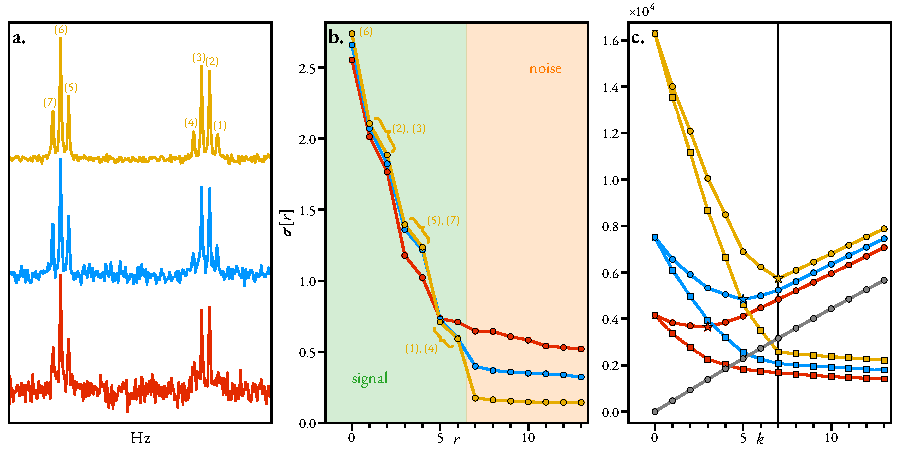
\includegraphics{mdl/mdl.pdf}
    \caption[
        An visualisation of the behaviour of the \acs{MDL} for three different
        \acsp{FID} comprising the same model, but with different noise variances.
    ]{
        An visualisation of the behaviour of the \acs{MDL} for three different
        \acsp{FID} comprising the same model, but with different noise
        variances. The model used to construct the \acp{FID} feature 7
        oscillators. The three \acsp{SNR} used were
        \qty{7}{\deci\bel} (red), \qty{12}{\deci\bel} (blue), and
        \qty{20}{\deci\bel} (yellow). The \acsp{FID} were generated with $\None
        = 256$.
        \textbf{a.} Spectra of the three \acsp{FID}.
        \textbf{b.} The values of the 14 most significant singular values
        associated with the Hankel matrix $\symbf{H}_{\symbf{Y}}$, with the
        pencil parameter $\Lone$ set to $\lfloor \nicefrac{\None}{3} \rfloor =
        85$).
        \textbf{c.} Square points with dotted lines: The negative log-likeliood
        \ac{MLE}, i.e. the first term of \eqref{eq:mdl}.
        Grey line: the penalty component of the \ac{MDL}, given by the second
        term in \eqref{eq:mdl}.
        Circular points with solid lines: the \ac{MDL}.
        Stars denote the minimum of the \ac{MDL} for a given \ac{FID}. The
        \qty{20}{\deci\bel}
        signal is correctly deemed to have a model order of 7, while the other
        two are underestimated (predicted models orders are 5 and 3 for the
        \qty{12}{\deci\bel} and \qty{7}{\deci\bel} \acsp{FID}, respectively).
    }
    \label{fig:mdl}
\end{figure}
Figure \ref{fig:mdl} illustrates the form of the \ac{MDL} for three signals
with equivalent underlying models, with $M=7$, and noise instances with
different variances. The first 14 singular values of $\symbf{H}_{\symbf{Y}}$
are plotted in panel b, where it can be seen that beyond the first 7, after
singular values accounting for signal components are accounted for, the
following singular values, associated with noise, decrease at a far slower
rate. The noise subspace for \acp{FID} with higher \acp{SNR} have singular
values which are (a) smaller in magnitude and (b) more consistent, such that
distinguishing the noise and signal subspaces is an easier task (cf. the
yellow line in panel b and the red line). As such, the \ac{MDL} is more likely
to provide a faithful estimate of the true number of components in the \ac{FID}
(panel c).

\note{Mention that multidimensional criteria are available, though not
implemented in this work.}

\section{\Acl{NLP} for NMR estimation}
\label{sec:nlp}
Attention now turns to the application of \acfi{NLP} in for \ac{FID}
estimation, which in this work accepts an initial guess of parameters from
the \ac{MPM}, $\symbf{\theta}^{(0)}$, and generates the final estimate,
$\bthstar$.

\subsection{An overview of \ac{NLP}}
\label{subsec:nlp-overview}
In an optimisation problem, the goal is to determine the minimum\footnote{
    In certain applications, the interest is actually in finding the maximum of
    a function. However, it is trivial to transform a maximisation problem into
    a minimisation problem by finding the minimum of negative of the function.
}
of a function $\Fth: \mathbb{R}^n \rightarrow \mathbb{R}, n \in \mathbb{N}$, often
called the \emph{cost function} or \emph{fidelity}.
This is typically with the goal of determining the argument $\bthstar$ at
which the optimum is found:
\begin{equation}
    \bthstar = \argmin_{\bth \in \mathbb{R}^n} \Fth.
    \label{eq:minF}
\end{equation}
The above problem is \emph{unconstrained}, as there are no limitations that the
parameter vector is subjected to. Unless $\Fth$ has particular properties, such
as convexity\footnote{
    A convex function is one such that a line segment through any two points of
    the function lies above it.
}, it is generally only possible to determine a \emph{local minimum},
rather than a \emph{global minimum}. $\bthstar$ is a local
minimiser of $\Fth$ if there is a \emph{neighbourhood} $V \ni \bthstar$ for which
\begin{equation}
    \Fthstar \leq \Fth\ \forall \bth \in V.
  \label{def:local-minimiser}
\end{equation}
$V \subset \mathbb{R}^n$ is such that one can move some amount in any direction
away from $\bthstar$ and still be in $V$.

Key to \ac{NLP} are the \emph{necessary conditions}, which define whether a
given vector $\bth$ is a local minimum of$\mathcal{F}$.
The \emph{first necessary condition} states
that if $\Fth$ is continuously differentiable, and $\bthstar$ is a local extremum of
$\Fth$, then the gradient vector $\bdgthstar \coloneq \nabla \Fthstar$ is the
zero vector:
\begin{equation}
    \bdgthstar = \symbf{0} \in \mathbb{R}^n
\end{equation}
The \emph{second necessary condition} subsequently states that
if $\Fth$ and $\bdgth$ are continuously differentiable, and $\bthstar$ is a
local minimiser of $\Fth$, then the Hessian matrix $\bdHthstar \coloneq
\nabla^2 \Fthstar$ is positive semidefinite, i.e.
\begin{equation}
  \symbf{v}^{\mathrm{T}} \bdHthstar \symbf{v} \geq 0\ \forall \symbf{v} \in \mathbb{R}^n.
\end{equation}
Furthermore, it is a \emph{unique} local minimiser if the \emph{second-order
sufficient condition} is also satisfied, i.e. that the Hessian is positive
definite:
\begin{equation}
    \symbf{v}^{\mathrm{T}} \bdHthstar \symbf{v} > 0\ \forall \symbf{v} \in \mathbb{R}^n.
\end{equation}

A plethora of approaches have been established to determine local minima of
scalar functions. One of the better-known strategies is \emph{Newton's method},
in which a quadratic approximation of the fidelity is considered.
For a given iteration $k \in \mathbb{N}_0$, the fidelity is approximated using
\begin{equation}
    \FQth =
        \Fthk +
        \symbf{h}\T \bdgthk +
        \tfrac{1}{2} \symbf{h}^{\mathrm{T}} \bdHthk \symbf{h},
    \label{eq:quad-approx}
\end{equation}
where $\symbf{h} = \bth - \bthk$.  An updated prediction of the parameter
vector is derived by finding the minimum of this quadratic approximation:
\begin{gather}
    \frac{\partial \Fth}{\partial \symbf{h}} =
        \bdgthk + \bdHthk \symbf{h} \notag\\
    \implies 0 = \bdgthk + \bdHthk \left(\bthkplusone - \bthk\right) \notag\\
    \therefore\ \bthkplusone =
        \bthk - \bdHthk^{-1}
        \bdgthk.\label{eq:newton-update}
\end{gather}
This process is repeated, until the convergence criterion as been met:
\begin{equation}
    \left\lVert \bdgthk \right\rVert \leq \epsilon.
\end{equation}
The threshold $\epsilon > 0$, can be tuned based on the desired accuracy of the
result, and is usually several order of magnitude less than $1$.
\Cref{eq:newton-update} tends not to be used as the update formula in real
optimisation problems. One of the major downsides of the Newton update is the
possibility that is not a minimising update if the Hessian is not positive
definite. Two primary strategies have emerged which are typically used instead:
\begin{itemize}
    \item \emph{Line search methods}\cite[Chapter 3]{Nocedal2006} determine an
        appropriate direction $\symbf{p}^{(k)}$ along which the updated
        parameter vector is sourced.  After this, an appropriate step length
        $\alpha^{(k)}$ is determined\,---\,typically in an efficient, though not
        optimal manner; abiding by the \emph{Wolfe conditions} is a common
        approach\,---\,leading to $\bthkplusone = \bthk -
        \alpha^{(k)}\symbf{p}^{(k)}$.
    \item \emph{Trust region methods}\cite[Chapter 4]{Nocedal2006} define a
        radius $\Updelta^{(k)} > 0$, and determine the minimum of
        \cref{eq:quad-approx} subject to the constraint that
        $\left\lVert\symbf{h}\right\rVert \leq \Updelta^{(k)}$.
\end{itemize}
A trust region method is applied in this work, and as such further
consideration of it will now be made.

\subsubsection{Trust Region Methods}

\begin{algorithm}
    \caption[
        Nonlinear programming routine employed in \acs{EsPy}.
    ]
    {
        Nonlinear programming routine employed in \acs{EsPy}. This makes use of
        Algorithms 4.1 \& 7.2 in \cite{Nocedal2006}, with a extra check
        inserted to deal with any negative-amplitude oscillators which may be
        generated as the routine evolves.
    }
    \label{alg:nlp}
    \begin{algorithmic}[1]
        \Procedure {NLP}{$\bY \in \mathbb{C}^{\None \times \cdots \times \ND}, \bthzero \in \mathbb{R}^{2(D + 1)M}$}
            \State $\trustradius{0} \gets \nicefrac{1}{10} \left\lVert \bdgthzeroY \right\rVert$;
            \State $\trmax \gets 16 \trustradius{0}$;
            \For {$k = 0, 1, \cdots $}
            \State $\symbf{p}^{(k)} \gets \textsc{SteihaugToint}\left(\symbf{Y}, \symbf{\theta}^{(k)}, \trustradius{k}\right)$;
                \Comment{See \cref{alg:steihaug-toint}}
                \State $\rho^{(k)} \gets
                    \frac
                        {\Fphithk - \Fphithkpk}
                        {\FphiQthk - \FphiQthkpk}$;
                \If {$\rho_k < \nicefrac{1}{4}$}
                \label{state:decrease-tr-start}
                \State $\trustradius{k+1} \gets \nicefrac{1}{4} \trustradius{k}$;
                    \label{state:decrease-tr-end}
                    \ElsIf {$\rho_k > \nicefrac{3}{4}$ \textbf{ and } $\left\lVert \symbf{p}^{(k)} \right\rVert = \trustradius{k}$}
                \label{state:increase-tr-start}
                \State $\trustradius{k+1} \gets \min\left(2 \trustradius{k}, \trmax\right)$;
                    \label{state:increase-tr-end}
                \Else
                \State $\trustradius{k+1} \gets \trustradius{k}$;
                \EndIf
                \If{$\rho^{(k)} > \nicefrac{3}{20}$}
                \label{state:large-rho-start}
                    \State $\bthkplusone \gets \bthk + \symbf{p}^{(k)}$;
                    \label{state:large-rho-end}
                \Else
                \label{state:small-rho-start}
                    \State $\symbf{\theta}^{(k+1)} \gets \symbf{\theta}^{(k)}$;
                    \label{state:small-rho-end}
                \EndIf
                \If{$k \bmod 25 = 0 \textbf{ and } \symbf{\theta}^{(k+1)}$ contains negative amplitudes}\label{state:neg-amp-start}
                    \State $\symbf{\theta}^{(0)} \gets \symbf{\theta}^{(k+1)}$ with negative-amplitude oscillators removed;
                    \State $\symbf{\theta}^{(*)}, \symbf{\epsilon}^{(*)} \gets \operatorname{NLP}\left(\symbf{Y}, \symbf{\theta}^{(0)}\right)$;
                \EndIf\label{state:neg-amp-end}
                \If{$\left\lVert \bdgthkplusone \right\rVert < \num[print-unity-mantissa=false]{1e-8}$}
                    \State \textbf{break};
                \EndIf
            \EndFor
            \State $\symbf{\theta}^{(*)} \gets \symbf{\theta}^{(k+1)}$
            \State $\symbf{\epsilon}^{(*)} \gets
                \sqrt{
                    \frac
                    {
                        \Fthstar \diag \left(
                            \left[\bdHthstar\right]^{-1}
                        \right)
                    }
                    {(\None \cdots \ND) - 1}
                }$
            \State \textbf{return} $\symbf{\theta}^{(*)}, \symbf{\epsilon}^{(*)}$;
        \EndProcedure
    \end{algorithmic}
\end{algorithm}

The structure of a typical trust region method is presented in
\cref{alg:nlp} (ignoring \crefrange{state:neg-amp-start}{state:neg-amp-end}, which is a custom addition,
see \cref{subsec:phase-variance}). An initial radius for the trust region
$\trustradius{0}$ is defined, along with a maximum permitted radius
$\trmax$, to ensure that excessively adventurous steps do not take place.
For each iteration $k$, a solution to the following sub-problem is sought:
\begin{equation}
    \begin{split}
        \bthkplusone = \argmin_{\bp \in \mathbb{R}^{n}}
            \Fthk +
            (\bthk + \bp)\T \bdgthk +
            \tfrac{1}{2} (\bthk + \bp)\T \bdHthk (\bthk + \bp) \\
        \text{subject to } \left \lVert \bp \right \rVert \leq \trustradius{k}.
    \end{split}
\end{equation}
This sub-problem is not usually minimised exactly, but instead an efficient
means of determining a sufficiently update is used.
Common approaches include computing the Cauchy point, the Dogleg
method, and a truncated conjugate-gradient
approach commonly called the \ac{ST} method\cite[Chapter 7]{Nocedal2006}.
The latter is employed in this work (see \cref{alg:steihaug-toint} and
\cref{lst:tr}). In the \ac{ST} approach, iterates of the conjugate-gradient
method\cite[Chapter 5]{Nocedal2006} are used, until either they go beyond the
trust region, or negative curvature is discovered.

Once a provisional update $\bthkplusone \coloneq \bth + \bpk$ is determined, a
metric is considered which indicates how effectively the quadratic estimate at
the proposed update $\bthkplusone = \bthk
+ \bpk$ agrees with the true value of the fidelity at this point:
\begin{equation}
    \rho^{(k)} = \frac
        {\Fthk - \Fthkpk}
        {\FQthk - \FQthkpk}.
\end{equation}
$\rho^{(k)}$ is the ratio between the actual reduction of the fidelity caused
by taking the proposed step, and the predicted reduction based on the quadratic
model. If $\rho^{(k)}$ is sufficiently close to $1$, the quadratic model being
used to generate new iterates is deemed to be acting well enough to warrant
accepting the proposed update
(\crefrange{state:large-rho-start}{state:large-rho-end}).
Furthermore, if $\rho^{(k)}$ is particularly close to 1, and the proposed
update is at the boundary of the trust radius, it is appropriate to enlarge the
radius of the trust region for the next iteration in an attempt to increase the
rate of convergence
(\crefrange{state:increase-tr-start}{state:increase-tr-end}).
On the other hand, a small value of $\rho^{(k)}$ implies that the
quadratic model reflects the true fidelity poorly, such that the proposed
update should be rejected
(\crefrange{state:small-rho-start}{state:small-rho-end}).
As well as this, the trust region's radius should be
decreased such that the model is more likely to behave faithfully
(\crefrange{state:decrease-tr-start}{state:decrease-tr-end}). The exact
thresholds which dictate whether to accept an update, and whether to adjust the
trust region radius are customisable. The hard-coded numerical values found in
\cref{alg:nlp} are the values used for the results acquired in this work.

\subsection{Non-linear programming applied to FID estimation}
\begin{remark}
    \label{rem:norm-data}
    Prior to estimating the dataset, it is normalised, such that the signal
    actually under consideration is $\nicefrac{\bY}{\lVert \bY \rVert}$.
    To make the result reflect the actual dataset, the final amplitudes $\bdastar$
    are multiplied by $\lVert \symbf{Y} \rVert$.
\end{remark}
Focussing now on the problem of FID estimation, the fidelity $\FthY
: \mathbb{C}^{\None \times \cdots \times \ND} \times
\mathbb{R}^{2(1 + D)M} \rightarrow \mathbb{R}$ is given by
\begin{equation}
    \FthY = \left \lVert \bY - \bXth \right \rVert^2.
    \label{eq:fidelity}
\end{equation}
The elements of the gradient vector $\bdgthY \in \mathbb{R}^{2(1+D)M}$ and
the Hessian matrix $\bdHthY \in \mathbb{R}^{2(1+D)M \times 2(1+D)M}$ are then
derived by taking the first and second partial derivatives of the fidelity with
respect to the elements in $\bth$, respectively:
\begin{subequations}
    \begin{gather}
        g_i = -2 \Re
                \left\langle
                    \left(\bY - \bX\right),
                    \frac{\partial \bX}{\partial \theta_i}
                \right\rangle,
        \label{eq:grad} \\
        h_{i,j} = 2 \Re
            \biggl(
                \underbrace{
                    \left\langle
                        \frac{\partial \bX}{\partial \theta_i},
                        \frac{\partial \bX}{\partial \theta_j}
                    \right\rangle
                }_{\circled{1}}
                -
                \underbrace{
                    \left\langle
                        \left(\bY - \bX\right),
                        \frac{\partial^2 \bX}{\partial \theta_i \partial \theta_j}
                    \right\rangle
                }_{\circled{2}}
            \biggl).
            \label{eq:hess}
    \end{gather}
    \label{eq:fidelity-grad-hess}
\end{subequations}
$\forall i,j \in \lbrace 1, \cdots, 2(1+D)M \rbrace$.
The complete set of first and second derivatives of a particular element of the
model $x \coloneq \xnonenD$, given by \cref{eq:x}, is as follows
$\forall m \in \lbrace 1, \cdots, M \rbrace$,
$\forall d, d^{\prime} \in \lbrace 1, \cdots, D \rbrace$:
\begin{subequations}
    \begin{gather}
        \xderiv{\theta_m} \equiv
            \xderiv{a_m} =
            \frac{x}{a_m},\\
        \xderiv{\theta_{m + M}} \equiv
            \xderiv{\phi_m} =
            \iu x,\\
        \xderiv{\theta_{m + (d + 1)M}} \equiv
            \xderiv{\fdm} =
            2 \pi \iu \Dtd \nd x,\\
        \xderiv{\theta_{m + (d + D + 1)M}} \equiv
            \xderiv{\etadm} =
            - \Dtd \nd x,\\
        \xderivtwosame{\theta_{m}} \equiv
            \xderivtwosame{a_m} =
            0,
            \label{eq:amp-second-deriv}\\
        \xderivtwodiff{\theta_{m}}{\theta_{m + M}} \equiv
            \xderivtwodiff{a_m}{\phi_m} =
            \frac{\iu x}{a_m},\\
        \xderivtwodiff{\theta_{m}}{\theta_{m + (d + 1)M}} \equiv
            \xderivtwodiff{a_m^{\vphantom{(d)}}}{\fdm} =
            \frac{2 \pi \iu \Dtd \nd x}{a_m},\\
        \xderivtwodiff{\theta_{m}}{\theta_{m + (d + D + 1)M}} \equiv
            \xderivtwodiff{a_m^{\vphantom{(d)}}}{\etadm} =
            \frac{-\Dtd \nd x}{a_m},\\
        \xderivtwosame{\theta_{m + M}} \equiv
            \xderivtwosame{\phi_m} =
            -x,\\
        \xderivtwodiff{\theta_{m + M}}{\theta_{m + (d + 1)M}} \equiv
            \xderivtwodiff{\phi_m^{\vphantom{(d)}}}{\fdm} =
            -2 \pi \Dtd \nd x,\\
        \xderivtwodiff{\theta_{m + M}}{\theta_{m + (d + D + 1)M}} \equiv
            \xderivtwodiff{\phi_m^{\vphantom{(d)}}}{\etadm} =
            -\iu \Dtd \nd x,\\
        \xderivtwodiff{\theta_{m + (d + 1)M}}{\theta_{m + (d^{\prime} + 1)M}} \equiv
            \xderivtwodiff{\fdm}{\fdmp} =
            -4\pi^2 \left(\Dtd \nd \right) \left(\Dtdp \ndp \right) x,\\
        \xderivtwodiff{\theta_{m + (d + 1)M}}{\theta_{m + (d^{\prime} + D + 1)M}} \equiv
            \xderivtwodiff{\fdm}{\etadmp} =
            -2 \pi \iu \left(\Dtd \nd \right) \left(\Dtdp \ndp \right) x,\\
        \xderivtwodiff{\theta_{m + (d + D + 1)M}}{\theta_{m + (d^{\prime} + D + 1)M}} \equiv
            \xderivtwodiff{\etadm}{\etadmp} =
            \left(\Dtd \nd \right) \left(\Dtdp \ndp \right) x,\\
        \xderivtwodiff{\theta_{i}}{\theta_{j}} =
            \xderivtwodiff{\theta_{j}}{\theta_{i}},
            \label{eq:symmetric-second-derivs}\\
        \xderivtwodiff{\theta_{i}}{\theta_{j}} = 0\ \text{ if not specified above.}
        \label{eq:zero-second-deriv}
    \end{gather}
\end{subequations}
\Cref{eq:zero-second-deriv} indicates that any second derivative
with respect to two parameters which do not belong to the same oscillator will
always be $0$. This, along with the symmetrical nature of the second derivatives, see
\cref{eq:symmetric-second-derivs}, drastically reduces the required
number of second derivatives to compute, from $4 (1 + D)^2 M^2$ per data-point
to  $(1+D)\left(3 + 2D\right)M$. Finally, \cref{eq:amp-second-deriv}
indicates that another $M$ second derivatives do not need to be computed. See
\cref{tab:number-of-derivatives} for the total number of derivatives that need
to be computed for signals with different numbers of dimensions.
\begin{table}
    \begin{center}
        \begin{tabular}{ c c c }
            \toprule
            dimensions &
                \# 1\textsuperscript{st} derivatives &
                \# 2\textsuperscript{nd} derivatives\\
            \midrule
            $1$ & $4M\None$ & $9M\None$\\
            $2$ & $6M\None\Ntwo$ & $20M\None\Ntwo$\\
            $3$ & $8M\None\Ntwo\Nthree$ & $35M\None\Ntwo\Nthree$\\
            $D$ &  $2(1 + D)M \None \cdots \ND$ &  $((1 + D)(2(1 + D) + 1) - 1)M \None\cdots\ND$\\
            \bottomrule
        \end{tabular}
    \end{center}
    \caption{
        The number of first and second derivatives that are necessary to
        compute both the gradient vector and Hessian matrix of the fidelity for
        1- 2- and 3-dimensional datasets, as well as a general $D$-dimensional
        dataset.
    }
    \label{tab:number-of-derivatives}
\end{table}

\subsection{Approximating the Hessian}
Despite many of the model second derivatives being $0$, computation of those
that are not zero, and subsequently using these the form the Hessian matrix, is
often the most computationally expensive part of the optimisation. There are a
large number of optimisation problems where this is the case, and as such
there is considerable precedent for improving the efficiency of optimisation
algorithms by generating approximations of the Hessian which are less expensive.
Examples include the \ac{GN} method and \ac{LM} algorithm,
which are specifically for residual sum-of-squares problems\cite[Chapter
10]{Nocedal2006}, as well as quasi-Newton methods such as the BFGS
method\cite[Chapter 6]{Nocedal2006}.

The \ac{GN} and \ac{LM} approaches replace the true Hessian matrix at each
iteration with the following expression:
\begin{equation}
    h_{i,j} \approx 2 \Re
        \left\langle
            \frac{\partial \bX}{\partial \theta_i},
            \frac{\partial \bX}{\partial \theta_j}
        \right\rangle,
    \label{eq:hess-approx}
\end{equation}
i.e. term \circled{2} in \cref{eq:hess} involving the second derivatives is
neglected. All that needs to be generated is the Jacobian
$\symbf{J} = \nicefrac{\partial \bX}{\partial \bth}$. This often
brings a very large reduction in the computational cost, as no extra
derivatives need to be computed for the Hessian at all, since the Jacobian is
already required for generating the gradient vector.
In situations where the residuals between the data and model are small, term
\circled{1} will tend to dominate term \circled{2}, and as such these methods
often enjoy a convergence rate close to that of Newton's method when close to
local minima. Despite this, by invoking this approximation, the rate of
convergence, i.e. the number of iterations required to reach $\bthstar$, tends
to be adversely affected. See \cref{subsec:optim-vis} for an example of
this phenomenon.

\subsection{Estimation Errors}
\label{subsec:errors}
The vector of standard errors associated with the \ac{NLP} routine is related
to the \emph{observed Fisher information matrix} at convergence\cite[Section
2.7]{Pawitan2001}:
\begin{equation}
    \symbf{\epsilon}\left(\bthstar\right) = \sqrt{\diag\left(\symbf{I}\left( \bthstar \right)^{-1}\right)},
\end{equation}
where the observed Fisher Information matrix contains the negative partial second
derivatives of the log-likelihood with respect to $\bth$:
\begin{equation}
    \symbf{I}\left(\bth\right)_{i, j} =
        -\frac
        {\partial^2 \ell \left( \bdthY \right)}
        {\partial \theta_i \partial \theta_j}.
\end{equation}
Recalling the form of the log-likelihood given by \cref{eq:log-likeihood},
the elements of $\symbf{I}\left(\bth\right)$ are
\begin{equation}
    \symbf{I}\left(\bth\right)_{i, j} =
        -\frac{1}{\sigma^2}
        \Re
        \biggl(
            \left\langle
                \frac{\partial \bX}{\partial \theta_i},
                \frac{\partial \bX}{\partial \theta_j}
            \right\rangle
            -
            \left\langle
                \left(\bY - \bX\right),
                \frac{\partial^2 \bX}{\partial \theta_i \partial \theta_j}
            \right\rangle
        \biggl),
\end{equation}
which very closely resembles the Hessian of $\bth$:
\begin{equation}
    \symbf{I}\left(\bth\right)_{i,j} =
        \frac{1}{2 \sigma^2} \left(
            \bdHth_{i,j}
        \right).
\end{equation}
The standard errors therefore take the form
\begin{equation}
    \symbf{\epsilon}\left(\bthstar\right) =
        \sqrt{
            2\sigma^2 \diag \left(
                \bdHthstar^{-1}
            \right)
        }.
\end{equation}
Considering that the mean and variance of the noise $\bW$ are $0$ and $2\sigma^2$, respectively:
\begin{equation}
    2 \sigma^2 = \frac{1}{\mathfrak{N} - 1}
    \left\lVert \bW \right\rVert^2 =
    \frac{1}{\mathfrak{N} - 1} \left \lVert
        \bY - \bXthstar
    \right \rVert^2,
\end{equation}
so that finally a useable expression for the standard errors is arrived at:
\begin{equation}
    \symbf{\epsilon}\left(\bthstar\right) =
        \sqrt{
            \frac
            {
                \Fthstar \diag \left(
                    \left[\bdHthstar\right]^{-1}
                \right)
            }
            {\mathfrak{N} - 1}
        }
\end{equation}

\subsection{Visualisation of a simple example}
\label{subsec:optim-vis}
\begin{figure}
    \centering
    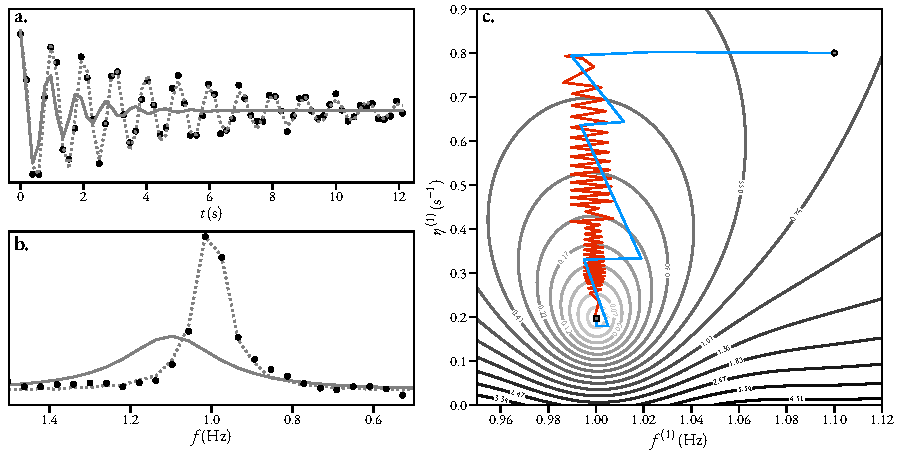
\includegraphics{optimisation_visualisation/optimisation_visualisation.pdf}
    \caption[
        A visualisation of the trajectory of a 2-parameter optimisation
        involving a simulated \acs{FID} comprising a single resonance.
    ]
    {
        A visualisation of the trajectory of a 2-parameter optimisation
        involving a simulated \acs{FID} comprising a single resonance.
        \textbf{a.} \& \textbf{b.} Representations of the signal in
        the time domain and Fourier domain, respectively.
        Black dots: the signal to be estimated $\bY$.
        Solid grey line: the model generated
        using the initial guess $\bX \left( \bthzero \right)$.
        Dotted grey line: the model generated using the optimised result, $\bX
        \left( \bthstar \right)$.
        \textbf{c.} A contour plot of the fidelity.
        Blue line: the trajectory of the parameter vector with the true
        Hessian matrix used in computing each update.
        Red line: the analogous trajectory using the Hessian approximation
        in place of the true Hessian.
    }
    \label{fig:optim-vis}
\end{figure}
\Cref{fig:optim-vis} provides a visualisation of numerical optimisation
applied on a simulated \ac{FID} comprising a single resonance.
The FID was constructed using \cref{eq:general-fid} with $D=1$, $M=1$,
$\None = 64$, $\fswone = \qty{5.2}{\hertz}$ ($\Dtone \approx
\qty{0.192}{\per\second}$), and $\foffone = \qty{0}{\hertz}$.
The resonance was parameterised by $\bth \in \mathbb{R}^4$ comprising $a=1$,
$\phi=\qty{0}{\radian}$, $\fone=\qty{1}{\hertz}$, $\etaone=\qty{0.2}{\per\second}$.
White Gaussian noise was added to the FID to give it \iac{SNR} of approximately
\qty{10}{\deci\bel}. As the visualisation of 5D space is beyond the scope of
this work, only two parameters, the frequency and damping factor were optimised
from an initial guess, with the amplitude and phase being fixed to their true
values. The initial guess comprised a frequency of \qty{1.1}{\hertz}, and a
damping factor of \qty{0.8}{\per\second}, with the solid grey lines in panels a
\& b denoting the model generated using the initial guess in the time- and
Fourier-domains, respectively. $\bthzero$ was subjected to \ac{NLP} twice. In
the first instance, the exact Hessian matrix, given by \cref{eq:hess} was used
in order to compute each update step, while in the second the Hessian
approximation given by \cref{eq:hess-approx} was used. The initial
radius of the trust region was set to $\nicefrac{1}{10}$ of the gradient norm
($\approx 0.3$), which has a precedent in the literature\cite{Gould2005}. The
trajectories of the parameter vector are denoted as coloured lines in panel c.
In both cases, the \ac{NLP} routine successfully generated a result $\bthstar$
in agreement with the true frequency and damping factor used to construct the
\ac{FID}. However, it is clear that using the true Hessian matrix (blue)
led to a far better rate of convergence compared with the
approximated analogue (red), which exhibited ``zig-zagging''. This phenomenon
is often seen in gradient descent methods, in which each update occurs in the
opposite direction to the gradient.
14 iterations were required to reach the
convergence criterion $\epsilon \leq \num[print-unity-mantissa=false]{1e-8}$
when the true Hessian was used, while 81 were required for the approximated
case. While an anecdotal example, this highlights that use of the true
Hessian matrix tends to allow a better rate of convergence. However, for
\acp{FID} comprising many signals and far more points, the approximated form
often requires a shorter time to converge overall, as the cost of computing the
second derivatives required for the true Hessian dominates.

\subsection{Phase Variance Minimisation}
\label{subsec:phase-variance}
\note{Re-write this section}
While numerical optimisation procedures can return estimates $\bthstar$ which
can achieve highly accurate reconstructions of the original \acs{FID} (i.e.
$\bY$ and  $\bXthstar$ are in close agreement), the estimate won't
necessarily provide a faithful description of the physical phenomenon that has
given rise to the data. For the purposes of \ac{FID} estimation, the goal is to
ensure that each signal contributing to the \ac{FID} is described by a
single oscillator in the model. In scenarios where the model order $M$ used is
greater than the true number of resonances, over-fitting of the data will
occur, leading to spurious features in the estimation result, such as single
resonances being fit by multiple oscillators and/or noise components being fit.
To overcome this problem, it is desirable to include known information about
the signal into the optimisation routine as a means of guiding the parameter
vector to a more appropriate final value. One particular means of achieving
this which has been to found to be effective is the incorporation of the
variance of oscillator phases into the fidelity, such that it becomes
\begin{equation}
    \FphithY = \left \lVert \bY - \bXth \right \rVert^2 + \circvar,
    \label{eq:fidelity-phasevar}
\end{equation}
where $\circvar$ is the \emph{circular variance} of the oscillator phases
(\textit{vide infra}).
\begin{remark}
    The inclusion of the phase variance into the fidelity is one of the
    motivating reasons for normalising the data prior to estimation (see
    \cref{rem:norm-data}). $\circvar$ is constrained to the interval $[0, 1]$.
    If the data were not normalised, it is likely that $\lVert \bY - \bX
    \rVert^2$ would dominate $\circvar$ in \cref{eq:fidelity-phasevar},
    such that the influence of the phase variance would be negligible.
\end{remark}
For the phase variance to act effectively, it is necessary to apply
phase-correction to the data prior to estimation, as the assumption that the
phases of all contributing resonances are equal is typically
valid.
\note{Mention phase-variation of multiplet peaks in experiments where
J-coupling evolves prior to acquisition? $T_2$ for example.}
The inclusion of phase variance has also been found to be effective at purging
excessive oscillators that may be present in the initial guess $\bthzero$,
which be thought of in the following way:
\begin{enumerate}
    \item Assume that the initial guess contains more oscillators than the
        true number of resonances. In this circumstance, it is common to find
        that true resonances are fit with an acceptable oscillator, whilst
        extra oscillators exist with spurious phases on account of
        over-fitting.
    \item Unconstrained numerical optimisation is now run, with the fidelity
        given by \cref{eq:fidelity-phasevar}. The phase variance will
        force oscillators with phases that are significantly different to the
        majority of oscillators to drastically alter their phases to match
        them. For some/all of these oscillators, it may be the case that the
        optimiser drives these to acquire a negative amplitude, such that they
        act as if they have a phase of $\pi$ while ensuring that $\circvar$ is
        small.
    \item This provides a criterion for detecting oscillators which are likely
        to be excessive. Such oscillators can be purged from $\bth$ by
        periodically checking whether any amplitudes (i.e. $\bth[:M]$) have
        become negative, purging these, and re-starting the optimisation.
    \item The numerical optimisation routine is re-started each time
        oscillators are purged. Termination is achieved once the routine
        converges and no negative-amplitude oscillators exist in $\bth$.
\end{enumerate}

\subsubsection{Circular Variance}
Oscillator phases are an example of a \emph{circular variable}, in that all
phases are wrapped within an interval of width $2 \pi$. Given an unconstrained
(unwrapped) phase $\widetilde{\phi} \in \mathbb{R}$, the corresponding wrapped
phase $\phi \in \left( -\pi, \pi \right]$ is given by
\begin{equation}
    \phi = \left(\left(\widetilde{\phi} + \pi\right) \bmod 2 \pi\right) - \pi.
    \label{eq:phase_wrap}
\end{equation}
This makes the conventional (linear)
definition of variance, given by
\begin{subequations}
    \begin{gather}
        \Var_{\shortmid}\hspace*{-3pt}\left(\symbf{\phi}\right) =
            \frac{1}{M} \sum_{m=1}^{M} \left(\phi_m - \mu\left(\symbf{\phi}\right)\right)^2, \\
        \mu\left(\symbf{\phi}\right) = \frac{1}{M} \sum_{m} \phi_m,
    \end{gather}
\end{subequations}
unsuitable for phases. Consider as a simple example a scenario
where there are two oscillators with phases $\widetilde{\bdphi} = \left[ \pi +
\delta\:\:\pi - \delta \right]\T$ for some small $\delta$.
The phase variance is expected to be small as these two phases are similar.
However, with the inclusion of wrapping through application of
\cref{eq:phase_wrap}, these phases would actually be set to $\bdphi = \left[
    -\pi
+ \delta\:\:\pi - \delta \right]\T$, and the conventional definition of phase
variance would be large. It is therefore apparent that a definition of variance
which accounts for the periodicity of the phases is needed. The \emph{circular
variance} is given by\cite[Chapter 3]{Fisher1993}
\begin{subequations}
    \begin{gather}
        [0, 1] \ni \circvar = 1 - \frac{R}{M},\\
        R = \sqrt{c_{\Sigma}^2 + s_{\Sigma}^2}, \\
        c_{\Sigma} = \sum_{m} \cos \phi_m, \\
        s_{\Sigma} = \sum_{m} \sin \phi_m.
    \end{gather}
\end{subequations}
$R$ is the length of the resultant vector produced by summing $M$ unit vectors
with the angles given by $\bdphi$. In the case that all the vectors have the
same angle, $R=M$, leading to the variance being $0$ as expected. At the other
extreme, with $M$ vectors uniformly separated about the unit circle (with an
angle $\nicefrac{2 \pi}{M - 1}$ between all pairs of adjacent vectors), the
vectors will perfectly cancel, leading to $R=0$. In this case, the maximum
variance of $1$ is obtained.

The first and second derivatives of the circular variance are required for
the computation of the gradient vector and Hessian matrix. These are given by
\begin{subequations}
    \begin{gather}
        \frac{\partial \circvar}{\partial \theta_i} =
        \begin{cases}
            \frac{1}{RM}
            \left(
                c_{\Sigma} \sin \phi_{i-M} -
                s_{\Sigma} \cos \phi_{i-M}
            \right) & M \leq i < 2M\\
            0 & \text{otherwise}
        \end{cases}\\
        \frac{\partial^2 \circvar}{\partial \theta_i \partial \theta_j} =
        \begin{cases}
            \begin{split}
                \tfrac{1}{RM}\left[
                    \tfrac{1}{R^2}
                    \left(c_{\Sigma} \sin \phi_{i-M}  - s_{\Sigma} \cos \phi_{i-M} \right)^2 \right. \\
                    \left. + c_{\Sigma} \cos \phi_{i-M} + s_{\Sigma} \sin \phi_{i-M}
                    - 1
                \vphantom{\tfrac{1}{RM}}\right]
            \end{split}
            & M \leq i, j < 2M, i = j\\
            \begin{split}
                \tfrac{1}{RM}\left[
                    \tfrac{1}{R^2}
                    \left(c_{\Sigma} \sin \phi_{i-M} - s_{\Sigma} \cos \phi_{i-M} \right) \right.\\
                    \times \left(c_{\Sigma} \sin \phi_{j-M} - s_{\Sigma} \cos \phi_{j-M} \right) \\
                    \left. - \cos\left( \phi_{i-M} - \phi_{j-M} \right)
                    \vphantom{\tfrac{1}{R^2}}
                \right]
            \end{split}
            & M \leq i, j < 2M, i \neq j\\
            0 & \text{otherwise}
        \end{cases}
    \end{gather}
\end{subequations}



\section{Profiling the Method}
\label{sec:profiling}
The routine described for \ac{FID} estimation involves operations which can be
computationally demanding, with the burden on resources
increasing with the number of points in the \ac{FID}, as well as the number of
oscillators in the model. This is the case both in terms of the amount of work
done by the \ac{CPU}, and the amount of \ac{RAM} needed to store all the
required data as the routine runs. For the matrix pencil methods, the most
demanding aspect is performing \ac{SVD}, while for \ac{NLP}, it
is generation of the Hessian matrix for each iteration. Detailed accounts of the
computational complexity of the \ac{MPM} and \ac{MMEMPM} have been
presented~\cite{Hua1992,Chen2007}.  However, it is useful to consider what the
actual run times of these routines are on a modern computer; a lot of
accounts on these are from decades before this work, and so the
run time will have decreased considerably thanks to
improvements in processing power. As an example, the account by Pines a
co-workers from 1997 outlining the \ac{ITMPM} states that a signal comprising
$1024$ points would take about
\qty{4.5}{\minute} to be processed by the \ac{MDL} and \ac{MPM}, using a
\qty{100}{\mega\hertz} \ac{CPU}~\cite{Lin1997}. On the system used for all
results generated for this work (see \cref{rem:workstation}) an
equivalent computation takes about \qty{100}{\milli\second}.

To derive the results presented in this section, \Python\ implementations of
the aforementioned parts of the estimation routine were run, with software used
to assess both the line-by-line execution times~\cite{LineProf}, and the
time-dependent \ac{RAM} usage~\cite{MemProf}.
\begin{remark}
    \label{rem:workstation}
    All results presented in this work were acquired using a workstation
    featuring a Intel\textregistered\ Core\texttrademark\ i9-10900X \ac{CPU} @
    \qty{3.7}{\giga\hertz}, and \qty{32}{\gibi\byte} of \ac{RAM}.
\end{remark}

\subsection{The \acs{MPM} and \acs{MMEMPM}}
\label{subsec:mpm-profiling}
\begin{figure}
    \centering
    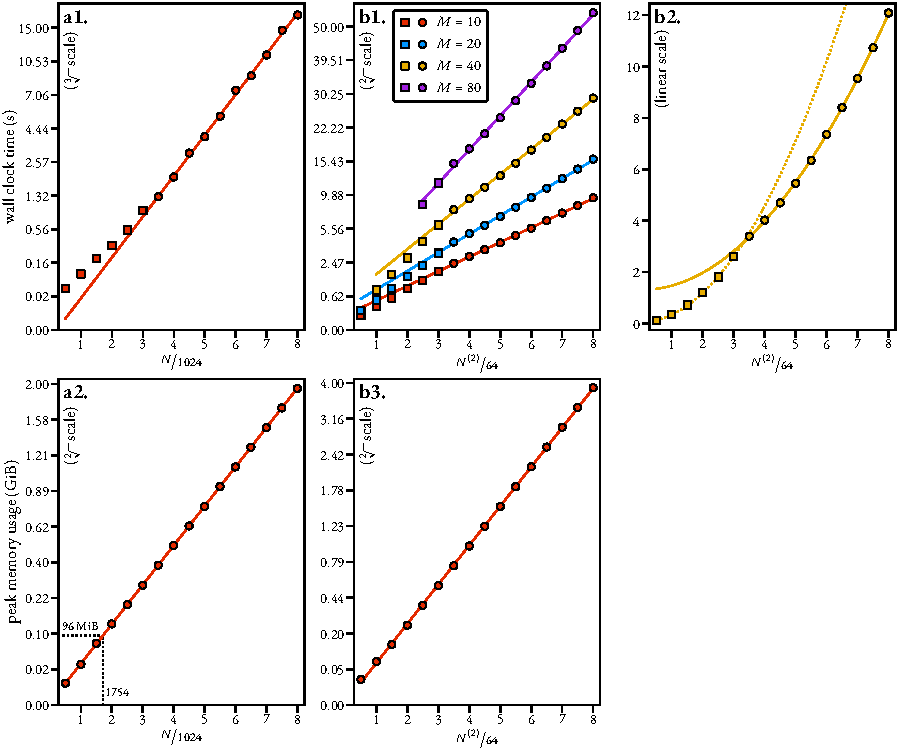
\includegraphics{mpm_profiling/mpm_profiling.pdf}
    \caption[
        The run time and peak memory consumption of
        the \acs{MPM} and \acs{MMEMPM}
        for \acsp{FID} with differing numbers of
        datapoints and constituent signals.
    ]
    {
        The run time and peak memory consumption of
        the \acs{MPM} and \acs{MMEMPM}
        for \acsp{FID} with differing numbers of
        datapoints and constituent signals.
        The \acp{FID} that were used to acquire these results are described in
        the main text.
        \textbf{a1.} The amount of time required to compute the \ac{MPM}, as a
        function of number of points. Also plotted is a cubic fit of the
        circular points.
        \textbf{a2.} Peak memory consumption in performing the \ac{MPM} as a
        function of the number of points.
        \textbf{b1.} The run time to compute the \ac{MMEMPM} of
        \acp{FID} with $\None = 64$, and variable $\Ntwo$ and $M$. Circular
        points have been fitted to quadratic functions.
        \textbf{b2.} The time required to compute the \ac{SVD} of $\EY$ for the
        $M=40$ \acp{FID}. The solid line is a quadratic fit of the circular
        points, while the dashed line is a quadratic fit of the square points.
        \textbf{b3.} Peak memory consumption in performing the \ac{MMEMPM} for
        the $M=40$ \acp{FID}.
    }
    \label{fig:mpm-profiling}
\end{figure}

A series of synthetic \ac{1D} \acp{FID} were constructed, comprising $10$ evenly-spaced
signals, with a
variable number of time-points $N \in \lbrace 512k : k \in \lbrace 1, 2, \cdots, 16 \rbrace \rbrace$.
For each \ac{FID}, the \ac{MPM} routine outlined in \cref{lst:mpm} was
performed 5 times.
The mean time to perform the \ac{MPM} across the 5 runs is plotted as a function
of $N$ in \cref{fig:mpm-profiling}.a1, where it can be seen that for
the larger values of $N$ considered, the \ac{MPM} is computed in approximately
$\mathcal{O}({N}^3)$ time;
a fit of a cubic function of the form $aN^3 + b$ to the data satisfying $7 \leq
k \leq 16$ is plotted to highlight this.
The cubic dependence is realised since the rate-limiting step of the
\ac{MPM} is \ac{SVD} of $\Hy$, whose size is to a very good approximation
$\tfrac{2N}{3} \times \tfrac{N}{3}$\footnote{
    \label{fn:svd-complexity}
    The time complexity for the \ac{SVD} of generic a $m \times n$ matrix is
    $\mathcal{O}(\operatorname{min}(m, n)^2 \cdot \operatorname{max}(m, n))$,
    while the space complexity is $\mathcal{O}(mn)$.
}. For smaller values of $N$, a deviation
away from a cubic relationship is observed.
This arises because the computation of the complex amplitudes using
\cref{eq:complex-amplitudes} has a comparatively significant run time
relative to \ac{SVD} in the low-$N$ regime;
for a $512$ point signal, \ac{SVD} of $\Hy$ took up roughly 80\% of the
complete run time, while the computation of the complex amplitudes took up
roughly 20\%. For a 8192 point signal, these percentages had changed to
$>\!\!99\%$ and $<\!\!1\%$, respectively.

The \ac{MPM} was run once more on each generated \ac{FID} in order to assess
the effect of $N$ on the space complexity.
The peak \ac{RAM} consumption is plotted in \cref{fig:mpm-profiling}.a2.
A clear quadratic dependence on consumption is realised as function of $N$,
again in agreement with the expected space complexity of the
\ac{SVD}\footnoteref{fn:svd-complexity}.

A similar study was conducted for the consideration of the \ac{MMEMPM}. A
series of hypercomplex \ac{2D} \acp{FID} were simulated, all of which all
comprised $\None = 64$. The \acp{FID} possessed values of $\Ntwo \in \lbrace
32k : k \in \lbrace 1, \cdots, 16 \rbrace \rbrace$.
With the \ac{MPM}, since a complete \ac{SVD} of the matrix $\Hy$ is computed,
the model order is irrelevant in dictating the run time (at least when $M \ll
N$). This is not the case for the \ac{MMEMPM}; because the \Python
implementation used (\cref{lst:mmempm}) employs a truncated \ac{SVD} in order
to compute only the first $M$ components of $\EY$, the elected model order will
have an impact on run time.  Therefore, \acp{FID} with different model orders
were generated: $M \in \lbrace 10, 20, 40, 80 \rbrace$.

The \ac{MMEMPM} was repeated 5 times for each \ac{FID}, and the mean run
times for each $\Ntwo$ and $M$ considered is plotted in
\cref{fig:mpm-profiling}.b1.
Results are only presented in cases where the \ac{MMEMPM} was able to yield a
satisfactory estimation result in close agreement with the model used to
generate the \ac{FID}; for certain \acp{FID} with low
$\Ntwo$ and high $M$, appropriate estimation results could not be obtained as
the constituent signals were too poorly resolved.
While in the high-$N$ regime the \ac{MPM} has a cubic time dependence
on the number of points, the \ac{MMEMPM} can be seen to have an approximately
quadratic complexity regarding $\Ntwo$.
For all combinations of $\Ntwo$ and $M$,
the truncated \ac{SVD} was the most time consuming aspect of the routine,
however other steps have notable run times too. The \ac{MMEMPM} can be broken
down into the following 5 steps, with the relevant lines in \cref{lst:mmempm}
given:
\begin{enumerate}
    \item Construction of $\EY$. This involves building the Hankel matrices
        $\lbrace \symbf{H}_{\symbf{y},\none} : \none \in \lbrace 0, \cdots, 63
        \rbrace \rbrace$, assigning them to the
        correct locations in $\EY$, and finally converting  $\EY$ to a sparse
        matrix\footnote{
            Truncated \ac{SVD} is only available for sparse matrices in
            \textsc{NumPy}~\cite{svds}. Some experimenting was done to determine
            the most efficient means of generating $\EY$ in sparse form, and
            subsequently compute its \ac{SVD}.
            It was determined that constructing $\EY$ using a
            standard \textsc{NumPy} array before converting it to
            \ac{CSR} format~\cite{csr} was optimal.
            \label{fn:sparse-svd}
        } (Lines \ref{ln:EYstart} to \ref{ln:EYend}).
    \item Truncated \ac{SVD} of $\EY$ to generate $\symbf{U}_M$ (Line \ref{ln:sparse2}).
    \item Determining $\bdzone$ and  $\symbf{W}^{(1)}$ by computing the
        eigenvalue decomposition of $\symbf{U}_{M1}^+ \symbf{U}_{M2}^{\vphantom{+}}$ (Lines
        \ref{ln:poles1start} to \ref{ln:poles1end}).
    \item Generating the second set of signal poles $\bdztwo$, by
        multiplying $\symbf{U}_M$ with the permutation matrix, and extracting
        the diagonal from matrix $\symbf{G}$, computed using \cref{eq:G} (Lines
        \ref{ln:poles2start} to \ref{ln:poles2end}). N.B. The \acp{FID} were
        constructed such that the signal poles were unique on all occasions, so
        the additional treatment of repeated signal poles was not necessary.
    \item Computation of the complex amplitudes using
        \cref{eq:complex-amplitudes-2d} (Lines \ref{ln:compamps2dstart} to
        \ref{ln:compamps2dend}).
\end{enumerate}
A comparison of the relative times to perform these steps for some select
pairings of $M$ and $\Ntwo$ is provided by \cref{tab:mmempm-steps}. It can be
seen that as $M$ increases, the relative amount of time spent performing
\ac{SVD} increases, while that to generate $\EY$ decreases. This
reflects the greater number of iterations required by
the truncated \ac{SVD} routine~\cite{svds} to produce the desired number of
components, while the run time to generate $\EY$ remains fixed.

Interestingly, the plots for a given value of $M$ in
\cref{fig:mpm-profiling}.b1 do not exhibit
consistent quadratic behaviour throughout; after a certain value of $\Ntwo$, a
slight reduction in the gradient of the plots is observed (cf
the square and circular points). This was found to be caused by the \ac{SVD}
computation, whose run times for the $M=40$ \acp{FID} are plotted in
\cref{fig:mpm-profiling}.b2.
The square and circular points both display quadratic behaviour, though the
exact form of the function which
describes them are different; both sets of points have been fit to curves of
the form $a\Ntwo^2 + b$. After $\Ntwo$ becomes larger than
roughly $200$, the \ac{SVD} run time appears to enter a new regime in which
a slower rate of increase is observed. The exact reason for why this is
observed was not ascertained.

The peak \ac{RAM} usage for the $M=40$ \acp{FID} as a function of $\Ntwo$ is
plotted in \cref{fig:mpm-profiling}.b3, where a quadratic complexity is
observed. The variation in memory consumption barely changes as a function of
the model order, since the peak usage is largely dependent on the size of
$\EY$.

It should be noted that the run time and peak \ac{RAM} consumption will also be
(roughly) quadratically dependent on $\None$, just as with $\Ntwo$, e.g.
increasing  $\None$ from  $64$ to $128$ would cause all the run times and peak
memory usages in Figures \ref{fig:mpm-profiling}.b1 and
\ref{fig:mpm-profiling}.b3 to quadruple in value.

\begin{table}
    \begin{center}
        \begin{tabular}{ c c c c c c c }
            \toprule
            $\Ntwo$ &
            $M$ &
            Step 1 &
            Step 2 &
            Step 3 &
            Step 4 &
            Step 5 \\
            \midrule
            64 & 10 & 12.2\% & 60.6\% & 2.9\% & 9.7\% & 13.8\% \\
            64 & 40 & 4\% & 74.6\% & 1.9\% & 8.9\% & 9.6\% \\
            512 & 10 & 22.1\% & 67.2\% & 0.2\% & 3.1\% & 7.2\% \\
            512 & 40 & 7.4\% & 81.9\% & 0.1\% & 1.3\% & 9.4\% \\
            512 & 80 & 3.8\% & 85.8\% & 0.1\% & 0.8\% & 9.4\% \\
            \bottomrule
        \end{tabular}
    \end{center}
    \caption[
        A comparison of the relative times to perform the steps in the \acs{MMEMPM}.
    ]{
        A comparison of the relative times to perform the steps in the
        \acs{MMEMPM}, for selected pairings on $M$ and $\Ntwo$. See the main
        text for a description of what each step entails.
    }
    \label{tab:mmempm-steps}
\end{table}

\subsection{Computing the Hessian for \acs{NLP}}
\begin{figure}
    \centering
    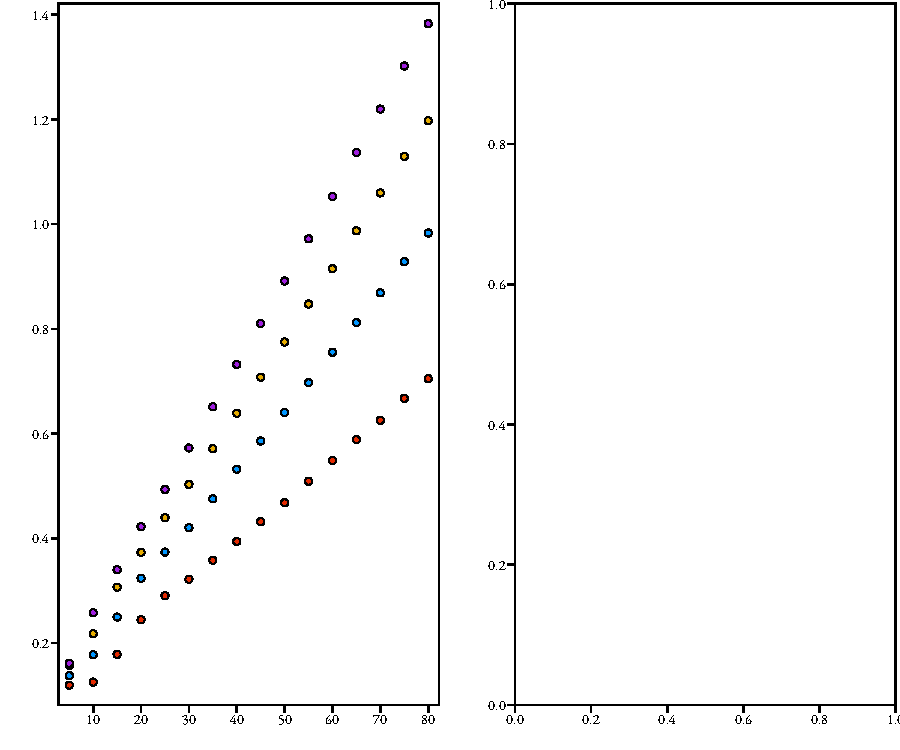
\includegraphics{nlp_profiling/nlp_profiling.pdf}
    \caption[
        The run time and peak memory consumption in computing the Hessian
        matrix for \acsp{FID} with differing numbers of datapoints and signals.
    ]
    {
        The run time and peak memory consumption in computing the Hessian
        matrix for \acsp{FID} with differing numbers of datapoints and signals.
        The \acp{FID} that were used to acquire these results are described in
        the main text.
        \textbf{a1.} and \textbf{b1.} The amount of time required to compute the
        Hessian for \ac{1D} and \ac{2D} \acp{FID}, respectively.
        \textbf{a2.} and \textbf{b2.} Equivalent plots showing the peak memory
        consumption in computing the Hessian.
    }
    \label{fig:nlp-profiling}
\end{figure}
A consideration of the burden on the \ac{CPU} and \ac{RAM} in computing the
Hessian matrix for \ac{1D} and \ac{2D} \acp{FID} (\cref{eq:hess}) is presented in
\cref{fig:nlp-profiling}.
It should be noted that for a typical \ac{NLP} routine, the Hessian will need
to be computed many times (on the order of magnitude of $10^2$ is common) so
while the times presented in the figure may seem small, a rather long total
time is possible for the \ac{NLP} routine if it takes seconds to compute the
Hessian once.
For the \ac{1D} case, simulated \acp{FID} were generated
with both a variable number of contributing signals: $M \in \lbrace 5k : k \in
\lbrace 1, 2, \cdots, 16 \rbrace \rbrace$ and datapoints: $N \in \lbrace 1024k
: k \in \lbrace 1, 2, \cdots, 8 \rbrace \rbrace$. For each \ac{FID}, the Hessian
was computed using a slight variant of the \texttt{obj\_grad\_hess\_1d}
function, given by Lines \ref{ln:objgradhessstart} to
\ref{ln:objgradhessend} in \cref{lst:obj-grad-hess}\footnote{
    The variant of this function neglected the computation of the objective and
    gradient, and returned only the Hessian.
}. There are 4 main steps in computing the Hessian matrix:
\begin{enumerate}
    \item Generation of all the first partial derivatives
        (\cref{eq:first-derivs}), which are stored in a $4M \times N$ array.
    \item Generation of all the non-trivially zero second partial
        derivatives (\cref{eq:second-derivs}), which are stored in a $10M
        \times N$ array.
    \item Computation of the non-zero elements of term \circled{2} in
        \cref{eq:hess}.
    \item Computation term \circled{1} in \cref{eq:hess}.
\end{enumerate}
These steps produce an exact Hessian. Neglecting steps 2 and 3 leads to the
formation of the approximated Hessian as described in
\cref{subsec:hess-approx}. \Cref{fig:nlp-profiling}.a1 shows that the
time to compute the Hessian matrix scales quadratically with $M$, and
linearly with $N$. The cause of this is the fact that the most time-consuming
aspect of the routine is step 4, which involves multiplying the $4M \times N$
matrix of first derivatives with its  $N \times 4M$ conjugate transpose, with a
complexity $\mathcal{O}(M^2N)$. The relative amount of the total run time which
is spent performing step 4 increases steadily as the model order increase, as
seen in \cref{tab:hess-steps}.
As such, for \ac{1D} \acp{FID}, it is
common, especially when the data comprises a large number of
signals, for the discrepancy in the amount of time to compute the true
Hessian relative to its approximation to be small. In these cases, it may be
valuable to compute the exact Hessian if it leads to a reduced number of
required iterations for convergence.
\begin{table}
    \begin{center}
        \begin{tabular}{ c c c c c c }
            \toprule
            $N$/$\Ntwo$ &
            $M$ &
            Step 1 &
            Step 2 &
            Step 3 &
            Step 4 \\
            \midrule
            \multicolumn{6}{c}{\textbf{1D Hessian}}\\
            \midrule
            2048 & 20 & 3.7\% & 9.6\% & 6\% & 76.4\% \\
            8192 & 20 & 3.5\% & 10.7\% & 6.3\% & 75\% \\
            2048 & 80 & 1\% & 3\% & 2\% & 92.6\% \\
            8192 & 80 & 1.2\% & 3.3\% & 1.9\% & 92.4\% \\
            \midrule
            \multicolumn{6}{c}{\textbf{2D Hessian}}\\
            \midrule
            64 & 20 & 8.2\% & 32.5\% & 18.5\% & 38.5\% \\
            256 & 20 & 12.3\% & 50.2\% & 21.3\% & 14.3\% \\
            64 & 80 & 10.8\% & 41\% & 24.3\% & 21.5\% \\
            256 & 80 & 14.9\% & 45.4\% & 24.1\% & 13.8\% \\
            \bottomrule
        \end{tabular}
    \end{center}
    \caption[
        A comparison of the relative times to perform the steps for
        computing the Hessian matrix for \acs{NLP}.
    ]{
        A comparison of the relative times to perform the steps for
        computing the Hessian matrix for \acs{NLP}, for selected pairings of
        $M$ and $N$ (\ac{1D})/$\Ntwo$ (\ac{2D}).
    }
    \label{tab:hess-steps}
\end{table}

To assess the effect of the number of signals and datapoints on Hessian
computation for \ac{2D} \acp{FID}, a series of signals were generated with a
fixed number of datapoints in the first dimension: $\None = 64$. \acp{FID} were
then constructed with the same values of $M$ as the \ac{1D} case, and $\Ntwo
\in \lbrace 64k : k \in \lbrace 1, 2, \cdots, 8 \rbrace \rbrace$. In contrast to
the \ac{1D} case, it is seen that the run time in computing the Hessian now
scales approximately linearly, rather than quadratically. Much more of the run
time is taken up by the first three steps in comparison; computing the
$6M\None\Ntwo$ first derivatives, $21M\None\Ntwo$ second derivatives, and
forming term \circled{2} all scale linearly with $M$, $\None$, and $\Ntwo$. The
relative times spent performing steps 2 and 3 compared with 1 and 4 imply that for
the \ac{2D} case (and for signals more more than 2 dimensions), a large saving
in computational time is typically achieved when the Hessian approximation
is utilised over the exact form.

Both the time- and space-complexity of computing the Hessian is found to be
roughly linear with both $M$ and the number of datapoints in each dimension
for \ac{1D} and \ac{2D} \acp{FID} (see Figures \ref{fig:nlp-profiling}.a2 and
\ref{fig:nlp-profiling}.b2). Most of the \ac{RAM} usage comes from storing
arrays of the first and second partial derivatives. In general, the typical
space requirements for both \ac{1D} and \ac{2D} \acp{FID} should be tolerable
on modern computers, which tend to possess at least \qty{8}{\gibi\byte} of
\ac{RAM}.

\section{Frequency Filtration}
\label{sec:filtering}
The previous section provides motivation for finding ways to reduce the
number of points in the signal and also the number of oscillators that the
signal contains. This has led to work on a procedure for generated
frequency-filtered ``sub-FIDs'' from the original data. A detailed description
of the filtering procedure is presented in this section.

\subsection{The \acl{VE}}
In brief, the filtering procedure  consists taking the \ac{FT} of the \ac{FID},
applying a band-pass filter on the spectral data to discard parts of not being
considered, and returning the spectrum back to the time-domain by an \ac{IFT}.
For a filtered \ac{FID} to be faithfully described by the model of a
summation of damped complex sinusoids, it is necessary that the
spectral peaks of interest lie effectively entirely within the filter
region\footnote{
    Lorentzian lineshapes tend to, but don't reach zero, as the distance from
    the maximum tends to $\infty$\cite{Tang1994}. However, as long as a
    sufficiently wide filtering is employed, the regions of the Lorentzian
    which do not pass through the filter can be assumed to be negligible.
}.
For absorptive Lorentzians, due to their characteristically narrow
linewidths, this is straightforward. However, for broader dispersive
Lorentzians, this is far more challenging. For this reason, generating
a spectrum in which only the real component is retained is desired.
Assuming the data has been phase-corrected, this will produce a
spectrum comprising only absorptive Lorentzians. The \ac{VE} has been employed
here, which has found application in the field of compressed sensing
NMR\cite{Mayzel2014,Golowicz2020,Luo2020}. This is a signal with double the
size as the original \ac{FID}, with the key characteristic that its \ac{FT} has
a real component which is equivalent to its counterpart derived from an
unaltered \ac{FID} (except it has double the points), and an imaginary
component of $0$s.

\subsubsection{The \acs{1D} \acl{VE}}
Assuming that a \ac{1D} \ac{FID} has been phase-corrected, such that $\bdphi =
\symbf{0} \in \mathbb{R}^M$, it can be denoted as
\begin{subequations}
    \begin{gather}
        \by =
        \symbf{\gamma} \odot
            \left(
                \symbf{c}^{(1)} + \iu \symbf{s}^{(1)}
            \right) + \bw, \\
        \symbf{\gamma} = \sum_m \bdam \exp \left(
                - \bdetaone \left[ m \right]
                \symbf{\tau}^{(1)}
            \right), \\
            \symbf{c}^{(1)}\text{/}\symbf{s}^{(1)} = \sum_m \cos\text{/}\sin \left(
                2 \pi \bdfone \left[ m \right] \symbf{\tau}^{(1)}_{\vphantom{t}}
            \right), \\
        \symbf{\tau}^{(1)} =
            \begin{bmatrix}
                0 & \Dtone & \cdots & \left(\None_{\vphantom{t}} - 1\right) \Dtone
            \end{bmatrix}\T
    \end{gather}
\end{subequations}
The frequency-dependence has been decomposed into its real and imaginary
components. With this in mind, a conjugate pair of signals are defined:
\begin{equation}
    \symbf{\psi}_{\pm} =
        \symbf{\gamma} \odot \left(
            \symbf{c}^{(1)} \pm \iu \symbf{s}^{(1)}
            \right) + \bw \equiv
            \Re\left(\by\right) \pm \iu \Im\left(\by\right)
\end{equation}
Two vectors $\lbrace \symbf{t}_{1}, \symbf{t}_2 \rbrace \in \mathbb{C}^{2
\None}$ are constructed using the conjugate pair:
\begin{itemize}
    \item $\symbf{t}_1$ is given by $\symbf{\psi}_+$ padded with zeros from below:
        \begin{equation}
            \symbf{t}_1 = \begin{bmatrix}
                \symbf{\psi}_+ \\ \symbf{0} \in \mathbb{C}^{\None}
            \end{bmatrix},\\
        \end{equation}
    \item $\symbf{t}_2$ is given by $\symbf{\psi}_{-}$ with its elements in
        reversed order ($\cdot^{{\leftrightsquigarrow}^{(1)}}$), padded with zeros
        from above, and finally subjected to a right circular shift by one
        element ($\cdot^{{\circlearrowright}^{(1)}}$):
        \begin{equation}
            \symbf{t}_2 = \begin{bmatrix}
                \symbf{0} \in \mathbb{C}^{\None} \\ \symbf{\psi}_-^{{\leftrightsquigarrow}^{(1)}}
        \end{bmatrix}^{{\circlearrowright}^{(1)}},
       \end{equation}
\end{itemize}
The \ac{VE} $\by_{\text{ve}}$ is then given by $\symbf{t}_1 +
\symbf{t}_2$, with the first element divided by $2$, which is equivalent to
\begin{equation}
    \by_{\text{ve}} =
    \begin{bmatrix}
        \Re\left( \by[0^{\vphantom{(1)}}] \right) &
        \by[1^{\vphantom{(1)}}] &
        \cdots &
        \by\left[\None - 1\right] &
        0 &
        \by\left[\None - 1\right]^* &
        \cdots &
        \by\left[1^{\vphantom{(1)}}\right]^*
    \end{bmatrix}\T.
\end{equation}
A signal of this form is illustrated in panel a of Figure \ref{fig:filtering}. As
eluded to already, the \ac{FT} of $\by_{\text{ve}}$ produces a spectrum
$\symbf{s}_{\text{ve}}$ such that $\Im\left(\symbf{s}_{\text{ve}}\right) =
\symbf{0}$, with $\Re\left(\symbf{s}_{\text{ve}}\right)$ featuring absorption
Lorentzian peaks (panel b of Figure \ref{fig:filtering}).


\subsubsection{The \acs{2D} \acl{VE}}
The \ac{VE} concept can be generalised to any number of dimensions, assuming
that a pair of amplitude-modulated signals exist for each indirect-dimension,
thus requiring a set of $2^{D-1}$ signals for a $D$-dimensional dataset.
\note{Maybe describe the general case in the appendix if you're bold enough?}
For the
\ac{2D} case, this corresponds to the pair of signals $\lbrace \bY_{\cos},
\bY_{\sin} \rbrace$, given by \eqref{eq:general-fid} with $D=2$ and $\zeta = \lbrace
\cos(\cdot), \sin(\cdot) \rbrace$, taking the forms (with noise neglected)
\begin{subequations}
    \begin{gather}
        \bY_{\cos} =
            \symbf{\Gamma} \odot
            \symbf{C}^{(1)} \odot \left(
                \symbf{C}^{(2)} +
                \iu \symbf{S}^{(2)}
            \right), \\
        \bY_{\sin} =
            \symbf{\Gamma} \odot
            \symbf{S}^{(1)} \odot \left(
                \symbf{C}^{(2)} +
                \iu \symbf{S}^{(2)}
            \right), \\
        \symbf{\Gamma} =
            \sum_m \bdam \left(
                \exp \left( -\bdetaonem \symbf{\tau}^{(1)} \right) \otimes
                \exp \left( -\bdetatwom \symbf{\tau}^{(2)} \right)
            \right), \\
        \symbf{C}^{(1)} \text{/} \symbf{S}^{(1)}
        = \sum_{m} \cos \text{/} \sin \left(2 \pi \bdfonem \symbf{\tau}^{(1)} \right)
            \otimes \symbf{1} \in \mathbb{C}^{\Ntwo}, \\
        \symbf{C}^{(2)} \text{/} \symbf{S}^{(2)} =
            \symbf{1} \in \mathbb{C}^{\None} \otimes
            \sum_{m} \cos \text{/} \sin \left(2 \pi \bdftwom \symbf{\tau}^{(2)} \right).
    \end{gather}
\end{subequations}
Four matrices are then constructed of the form
\begin{equation}
    \begin{gathered}
        \symbf{\Psi}_{\pm\pm} =
            \symbf{\Gamma} \odot \left(
                \symbf{C}^{(1)} \pm^{(1)} \hspace*{2pt} \iu \symbf{S}^{(1)}
                \right) \odot \left(
                    \symbf{C}^{(2)} \pm^{(2)} \hspace*{2pt} \iu \symbf{S}^{(2)}
                \right) \\
         \equiv
             \Re\left( \symbf{Y}_{\cos} \right)
             \pm^{(1)} \pm^{(2)} -
             \Im\left( \symbf{Y}_{\sin} \right)
             + \iu \left(
             \pm^{(1)}
             \Re\left( \symbf{Y}_{\sin} \right)
             \pm^{(2)}
             \Im\left( \symbf{Y}_{\cos} \right)
             \right),
    \end{gathered}
\end{equation}
from which the matrices $\symbf{T}_{1 \rightarrow 4} \in \mathbb{C}^{2 \None
\times 2 \Ntwo}$ are generated:
\begin{subequations}
    \begin{gather}
        \symbf{T}_1 =
        \begin{bmatrix}
            \symbf{\Psi}_{++} & \symbf{0} \\
            \symbf{0} & \symbf{0}
        \end{bmatrix}, \\
        \symbf{T}_2 =
        \begin{bmatrix}
            \symbf{0} & \symbf{0} \\
            \symbf{\Psi}_{-+}^{\leftrightsquigarrow (1)} & \symbf{0}
        \end{bmatrix}^{\circlearrowright (1)}, \\
        \symbf{T}_3 =
        \begin{bmatrix}
            \symbf{0} & \symbf{\Psi}_{+-}^{\leftrightsquigarrow (2)} \\
            \symbf{0} & \symbf{0}
        \end{bmatrix}^{\circlearrowright (2)}, \\
        \symbf{T}_4 =
        \begin{bmatrix}
            \symbf{0} & \symbf{0} \\
            \symbf{0} & \symbf{\Psi}_{--}^{\leftrightsquigarrow (1,2)}
        \end{bmatrix}^{\circlearrowright (1,2)}.
    \end{gather}
\end{subequations}
\note{Appendix for explicit forms of the matrices $\symbf{T}_{1-4}$}
The virtual echo is then given by $\symbf{Y}_{\text{ve}} = \sum_{i=1}^4
\symbf{T}_i$, with the first row and column divided by two. For a full outline
of the 2D filtering procedure, see Algorithm \ref{alg:filter-2d}.

It is possible to construct a virtual echo using an appropriate set of
phase-modulated signals too, which for the \ac{2D} case would be $\lbrace
\symbf{Y}_{\text{pos}}, \symbf{Y}_{\text{neg}}\rbrace$, given by
\eqref{eq:general-fid} with $D=2$ and  $\zeta = \lbrace \exp(\iu \cdot),
\exp(-\iu\cdot)\rbrace$. These can be used to generate an amplitude modulated pair via
\begin{subequations}
    \begin{gather}
        \symbf{Y}_{\text{cos}} = \frac{\symbf{Y}_{\text{pos}} + \symbf{Y}_{\text{neg}}}{2},\\
        \symbf{Y}_{\text{sin}} = \frac{\symbf{Y}_{\text{pos}} - \symbf{Y}_{\text{neg}}}{2\iu}.
    \end{gather}
\end{subequations}
\note{Should give $\zeta$ a dimension index, i.e.  $\zeta^{(1)}$}

\subsection{The filtering process}
Having constructed a virtual echo $\symbf{Y}_{\text{ve}} \in \mathbb{C}^{2\None
\times \cdots \times 2\ND}$, a spectrum with absorption Lorentzians is produced
with $\symbf{S}_{\text{ve}} = \FT\left(\symbf{Y}_{\text{ve}}\right)$. To filter
the spectrum, it is subjected to element-wise multiplication with a
super-Gaussian function. The super-Gaussian is defined by a centre
$c^{(d)} \in \mathbb{R}: 0 < c^{(d)} < 2 \Nd$ and a bandwidth  $b^{(d)} \in
\mathbb{N}: b^{(d)} < 2\Nd$ in each dimension (panel c of Figure
\ref{fig:filtering}):
\begin{subequations}
    \begin{gather}
        \symbf{G} = \bigotimes_{d=1}^D
            \symbf{g}^{(d)}, \\
        \symbf{g}_{\vphantom{t}}^{(d)}\left[ \nd \right] = \exp \left(
            -2^{p+1} \left(
                \frac{\nd - c^{(d)}_{\vphantom{t}}}{b^{(d)}}
            \right)^p
        \right)\ \forall \nd \in \lbrace 0, \cdots, 2 \Nd - 1 \rbrace.
        \label{eq:super-Gaussian-onedim}
    \end{gather}
\end{subequations}
An example of a \ac{1D} super-Gaussian is given in panel $c$ of Figure
\ref{fig:filtering}. The scalar $p \in \mathbb{R}_{>0}$ dictates the steepness
of the filter at the boundaries, with the function becoming more ``box-like''
as it increases. It is set to $40$ in this work and as the default in
\ac{EsPy}. Application of the super-Gaussian filter to $\symbf{S}_{\text{ve}}$
would lead to large sections of the filtered spectrum being $0$. This has an
undesired impact on the \ac{MDL}, as noise that has passed through filter (i.e.
the noise inside the region of interest) will now seem to resemble true signal,
as its amplitude is infinitely greater than the zeroed regions. A massive
over-estimation of model order therefore result. In order to obtain better
results from the model order selection, an array of synthetic \ac{AWGN} is
added to the filtered spectrum. To achieve this, a region in
$\symbf{S}_{\text{ve}}$ is specified which contains no discernible signal peaks
(referred to as the \emph{noise region}). The variance of this region
$\sigma^2$ is determined, and used to construct an array of values sampled from
a normal distribution with mean $0$ and variance $\sigma^2$,
$\symbf{W}_{\sigma^2} \in \mathbb{R}^{2 \None \times \cdots \times 2 \ND}$.
The filtered spectrum is then given by
\begin{equation}
    \widetilde{\symbf{S}}_{\text{ve}} = \symbf{S}_{\text{ve}} \odot \symbf{G} + \symbf{W}_{\sigma^2} \odot \left(\symbf{1} - \symbf{G} \right).
    \label{eq:Sve-tilde}
\end{equation}
Note that the noise array's magnitude at each point is attenuated by the value
of the super-Gaussian filter. Inside the region of interest ($\symbf{G}\left[
\none, \cdots, \nD \right] = 1$ ), the noise is nullified. See panel d of
Figure \ref{fig:filtering} for an example.

After filtering, $\widetilde{\symbf{S}}_{\text{ve}}$ is returned to the
time-domain by \ac{IFT}. The \ac{IFT} of a real-valued spectrum generates a
conjugate-symmetric signal. This is sliced in half in each dimension,
generating the final filtered sub-FID $\widetilde{\bY} \in
\mathbb{C}^{\None \times \cdots \times \ND}$:
\begin{equation}
    \widetilde{\bY} =
        \frac{1}{2^{D-1}}
        \IFT\left(\widetilde{\symbf{S}}_{\text{ve}}\right)
        \left[0:\None, \cdots, 0:\ND\right].
        \label{eq:yve-tilde}
\end{equation}
The scaling factor in \eqref{eq:yve-tilde} is to account for how many signals
have been combined to generate the \ac{VE}.

\begin{figure}
     \centering
     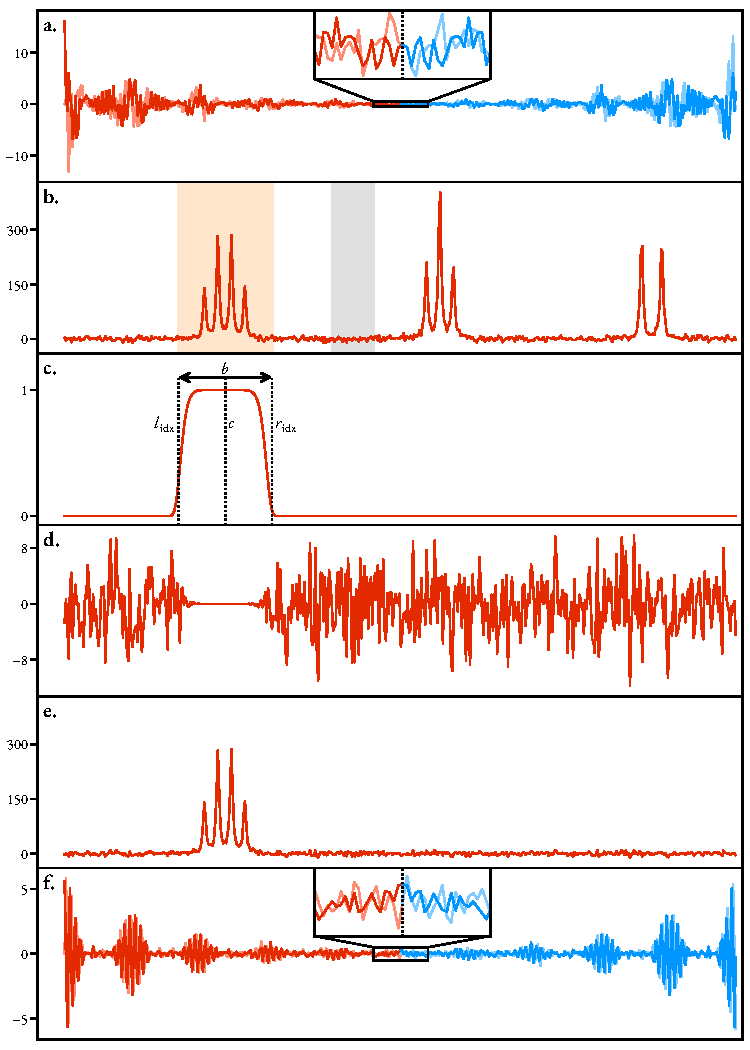
\includegraphics{filtering/filtering.pdf}
     \caption[
         An illustration of the filtering procedure applied to a \acs{1D}
         \acs{FID}.
     ]{
         An illustration of the filtering procedure applied to a \ac{1D}
         \ac{FID}.
         \textbf{a.} A \ac{VE} $\by_{\text{ve}}$, with the first and last
         $\None$ points coloured red and blue, respectively. The middle of the
         \ac{VE} is magnified to highlight its conjugate symmetry.
         \textbf{b.} The \ac{FT} of the \ac{VE}, $\symbf{s}_{\text{ve}}$.
         The region of interest (orange) and noise region (grey) are denoted.
         \textbf{c.} A super-Gaussian function used as a band-pass filter,
         $\symbf{g}$.
         \textbf{d.} \acs{AWGN} vector to be added to the filtered spectrum.
         The magnitude of the signal at each point is dependent on the
         corresponding super-Gaussian value.
         \textbf{e.} The filtered spectrum $\widetilde{\symbf{s}}_{\text{ve}}$,
         formed by applying the super-Gaussian filter, and adding the noise
         vector.
         \textbf{f.} The \ac{IFT} of the filtered spectrum,
         $\widetilde{\symbf{y}}_{\text{ve}}$, from which the final filtered
         signal $\widetilde{\symbf{y}}$ is obtained by extracting
         the first $\None$ points.
     }
     \label{fig:filtering}
\end{figure}

\subsubsection{Determining $c^{(d)}$ and  $b^{(d)}$}
The central index and bandwidth of the super-Gaussian filter function are given by the following expressions:
\begin{subequations}
    \begin{gather}
        c_{\vphantom{\text{idx}}}^{(d)} = \tfrac{1}{2} \left(l^{(d)}_{\text{idx}} + r^{(d)}_{\text{idx}}\right), \\
        b_{\vphantom{\text{idx}}}^{(d)} = l^{(d)}_{\text{idx}} - r^{(d)}_{\text{idx}},
    \end{gather}
\end{subequations}
where $l^{(d)}_{\text{idx}}$ and $r^{(d)}_{\text{idx}}$ denote the desired
indices where the filter's left and right bounds are located, respectively.
Array indices can be obtained from the corresponding spectral frequency
$f^{(d)}_{\unit{\hertz}}$ via
\begin{equation}
    \begin{gathered}
        f_{\text{idx}}^{(d)} =
            \left \lfloor
                \frac
                {
                    \left(2 \Nd_{\vphantom{d}} - 1\right)
                    \left(\fswd + 2 \left(\foffd - f_{\unit{\hertz}}^{(d)}\right) \right)
                }
                {2 \fswd}
            \right \rceil \\
        \forall f^{(d)}_{\unit{\hertz}} \in
            \left[\foffd - \tfrac{1}{2} \fswd, \foffd + \tfrac{1}{2} \fswd\right].
        \label{eq:fidx}
    \end{gathered}
\end{equation}
Conversion from \unit{\partspermillion} to array indices can be achieved by
replacing  $f_{\unit{\hertz}}$ in \eqref{eq:fidx} with
$f_{\unit{\partspermillion}} f_{\text{sfo}}$, where $f_{\text{sfo}}$ is the
transmitter frequency (\unit{\mega \hertz}).

\subsubsection{Spectrum slicing}
Thus far, the method described is able to reduce the model order of a given
signal, however the signal still comprises the same number of points. However
it is clear that there are a large number of points outside the region of
interest in $\widetilde{\symbf{S}}_{\text{ve}}$ that do not possess any
meaningful information. Discarding such points should then lead to filtered
\ac{FID} with the same information about the resonances of interest, but with
far fewer points. A slicing ratio is defined, $\xi \in \mathbb{R}: \xi > 1$,
which dictates the left and right indices at which the spectrum should be sliced
in each dimension:
\begin{subequations}
    \begin{gather}
        l_{\text{slice}}^{(d)} =
        \begin{cases}
            c_{\text{idx}}^{(d)} - \left \lfloor \frac{b^{(d)} \xi}{2} \right \rfloor &
            \text{if } \geq 0 \\
            0 & \text{otherwise}
        \end{cases} \\
        r_{\text{slice}}^{(d)} =
        \begin{cases}
            c_{\text{idx}}^{(d)} + \left \lceil \frac{b^{(d)} \xi}{2} \right \rceil &
            \text{if } \leq 2 \Nd - 1 \\
            2 \Nd - 1 & \text{otherwise}
        \end{cases}
    \end{gather}
\end{subequations}
The filtered spectrum is then sliced accordingly:
\begin{equation}
    \widetilde{\symbf{S}}_{\text{ve, slice}} =
        \widetilde{\symbf{S}}_{\text{ve}} \left[
            l_{\text{slice}}^{(1)} :
            r_{\text{slice}}^{(1)} + 1,
            \cdots,
            l_{\text{slice}}^{(D)} :
            r_{\text{slice}}^{(D)} + 1
        \right].
\end{equation}
The equivalent process is applied to $\widetilde{\symbf{S}}_{\text{ve,slice}}$
to generate the final filtered sub-\ac{FID}: \ac{IFT} followed by slicing in
half in each dimension.  It is also necessary to scale the signal by the ratio
of the number of points in the sliced spectrum and it's unsliced counterpart.
\begin{subequations}
    \begin{gather}
        \widetilde{\bY} =
            \prod_{d=1}^D \left(\frac{r_{\text{slice}}^{(d)} - l_{\text{slice}}^{(d)}}{2 \Nd}\right)
            \IFT \left( \widetilde{\symbf{S}}_{\text{ve, slice}} \right)
            \left[
                0 : \None_{\text{slice}}, \cdots, 0 : \ND_{\text{slice}}
            \right] \\
            \Nd_{\text{slice}} = \left \lfloor \frac{r_{\text{slice}}^{(d)} - l_{\text{slice}}^{(d)}}{2} \right \rfloor
    \end{gather}
\end{subequations}
Finally, the effective sweep widths and transmitter offsets will have been
altered by this process. The corrected values can be computed using
\begin{subequations}
    \begin{gather}
        f_{\text{sw,slice}}^{(d)} = \frac{r_{\text{slice}}^{(d)} - l_{\text{slice}}^{(d)}}{2 \Nd - 1} \fswd \\
        f_{\text{off,slice}}^{(d)} = \foffd + \frac{\fswd}{2} \left( 1 - \frac{l_{\text{slice}}^{(d)} + r_{\text{slice}}^{(d)}}{2 \Nd - 1}\right)
    \end{gather}
\end{subequations}

\section{Summary}
The \ac{MPM} is well established as an effective method for the parametric
estimation of signals in a number of disciplines.
One notable downside of the technique that has been realised while assessing
its effectiveness in parametrising \ac{NMR} \acp{FID} is its propensity to
return oscillators with unexpected phase behaviour, especially in scenarios
involving signals with similar frequencies, exhibiting considerable overlap in
the Fourier domain.
For this reason, using the result of the \ac{MPM} as an initial guess to feed
into a phase-variance regularised \ac{NLP} routine is proposed as a means of
returning improved parameter estimates. The theory underpinning the procedure
has been explored in this chapter.

The computational burden of running the procedure is large and often
insurmountable for complete \ac{NMR} datasets, which commonly comprise thousands of
points, and at least hundreds of contributing signals. Both the run time
and peak memory consumption of the \ac{1D} and \ac{2D} methods increase for \acp{FID} with more datapoints and more signals.
For this reason, a method to break the estimation problem into a
series of smaller, computationally tractable problems, through the construction
of frequency-filtered sub-\acp{FID}, has been introduced.

Having established an estimation routine, the next chapter focusses on its
performance in analysing \ac{1D} \ac{NMR} datasets, along with two specific
applications that arise.

% Algorithm \ref{alg:1d-2d-summary} provides an overview of the principal steps
% involved in the \ac{1D} estimation procedure. Detailed algorithms for each step
% are presented elsewhere in this text.

% \begin{algorithm}
%     \begin{algorithmic}[1]
%         \caption[
%             An overview of the estimation procedure outlined in this work.
%         ]{
%             An overview of the estimation procedure outlined in this work, for
%             the consideration of \ac{1D} \acp{FID}.
%         }
%         \label{alg:1d-2d-summary}
%         \Procedure{Estimate$1$D}{$
%             \by \in \mathbb{C}^{\None},
%             \symbf{R}_{\text{interest}} \in \mathbb{R}^{K \times 2},
%             \symbf{r}_{\text{noise}} \in \mathbb{R}^{2},
%             M \in \mathbb{N}_0
%             $
%         }
%             \State $l_{\text{idx,noise}}, r_{\text{idx,noise}} \gets r_{\text{noise}, 1}, r_{\text{noise}, 2}$;
%             \For{$k = 1, \cdots, K$}
%                 \State $l_{\text{idx}}, r_{\text{idx}} \gets r_{\text{interest}, k, 1}, r_{\text{interest}, k, 2}$;
%                 \State $\widetilde{\by} \gets \textsc{Filter}1\textsc{D}\left(
%                     \by,
%                     \right)
%                 $;
%                 \Comment{Algorithm \ref{alg:filter-1d}}
%                 \If{$M=0$}
%                     \State $M \gets \textsc{MDL}\left(\widetilde{\symbf{y}}\right)$;
%                     \Comment{\note{TODO}}
%                 \EndIf
%                 \State $\bthzero \gets \textsc{MPM}\left(\widetilde{\by}, M\right)$;
%                 \Comment{Algorithm \ref{alg:mpm}}
%                 \State $\bthstar, \symbf{\epsilon}^{(*)} \gets \textsc{NLP}\left(\widetilde{\by}, \bthzero\right)$;
%                 \Comment{Algorithm \ref{alg:nlp}}
%                 \State \textbf{return} $\bthstar, \symbf{\epsilon}^{(*)}$;
%             \EndFor
%         \EndProcedure
% %         \Statex
% %         \Procedure{Estimate$2$D}{$
% %             \bY_{\cos} \in \mathbb{C}^{\None \times \Ntwo},
% %             \bY_{\sin} \in \mathbb{C}^{\None \times \Ntwo},
% %             \symbf{R}_{\text{interest}} \in \mathbb{R}^{2 \times 2},
% %             \symbf{R}_{\text{noise}} \in \mathbb{R}^{2 \times 2},
% %             M \in \mathbb{N}_0
% %             $
% %         }
% %             \State $\widetilde{\bY} \gets \textsc{Filter}2\textsc{D}\left(
% %                 \bY_{\cos},
% %                 \bY_{\sin},
% %                 \symbf{R}_{\text{interest}},
% %                 \symbf{R}_{\text{noise}}
% %                 \right)
% %             $;
% %             \Comment{Algorithm \ref{alg:filter-2d}}
% %             \If{$M=0$}
% %                 \State $M \gets \textsc{MDL}\left(\widetilde{\bY}[:, 0]\right)$;
% %                 \Comment{Run the MDL on the first direct-dimension slice.}
% %             \EndIf
% %             \State $\bthzero \gets \textsc{MMEMPM}\left(\widetilde{\bY}, M\right)$;
% %             \Comment{Algorithm \ref{alg:mmempm}}
% %             \State $\bthstar, \symbf{\epsilon}^{(*)} \gets \textsc{NLP}\left(\widetilde{\bY}, \bthzero\right)$;
% %             \Comment{Algorithm \ref{alg:nlp}}
% %             \State \textbf{return} $\bthstar, \symbf{\epsilon}^{(*)}$;
% %         \EndProcedure
%     \end{algorithmic}
% \end{algorithm}


